
Este manual abarca toda la funcionalidad de la herramienta en cuanto a gestión
de personal, actividades y a la interacción ambos, aparte de los informes que
pueden generarse. El acceso a la aplicación no forma parte de este manual, por
lo que deberá consultarse el manual de usuario existente antes de que se
introdujeran las nuevas funcionalidades.

\section{Gestión de personal}
\label{sec:manual_personal}

Para una gestión integral del personal, debemos ser capaces de introducir nuevo
personal, modificar personal existente y borrar personal. Parte de su
información varía de forma periódica, en general, anualmente, por lo que
también se guiará a través del proceso de gestión de esta información.

Para comenzar a gestionar recursos, lo primero que debemos hacer es seleccionar
la entrada del menú con el nombre \textbf{Personal}, como se ve en la figura
\ref{fig:inicio_manual}.

\begin{figure}
\centering
\epsfig{file=imagenes/manual/inicio.eps,width=5.28in}
\caption{Enlace al módulo de personal en el menú.}
\label{fig:inicio_manual}
\end{figure}

\subsection{Búsqueda de personal}
\label{sec:manual_busqueda_personal}

Lo primero que nos encontramos es un buscador de personal (figura
\ref{fig:filtro_personal}), que funciona más propiamente como un filtro: esto
quiere decir que si no introducimos ningún valor y pulsamos \textbf{Buscar}, se
nos mostrarán todos los empleados de todas las empresas.

\begin{figure}
\centering
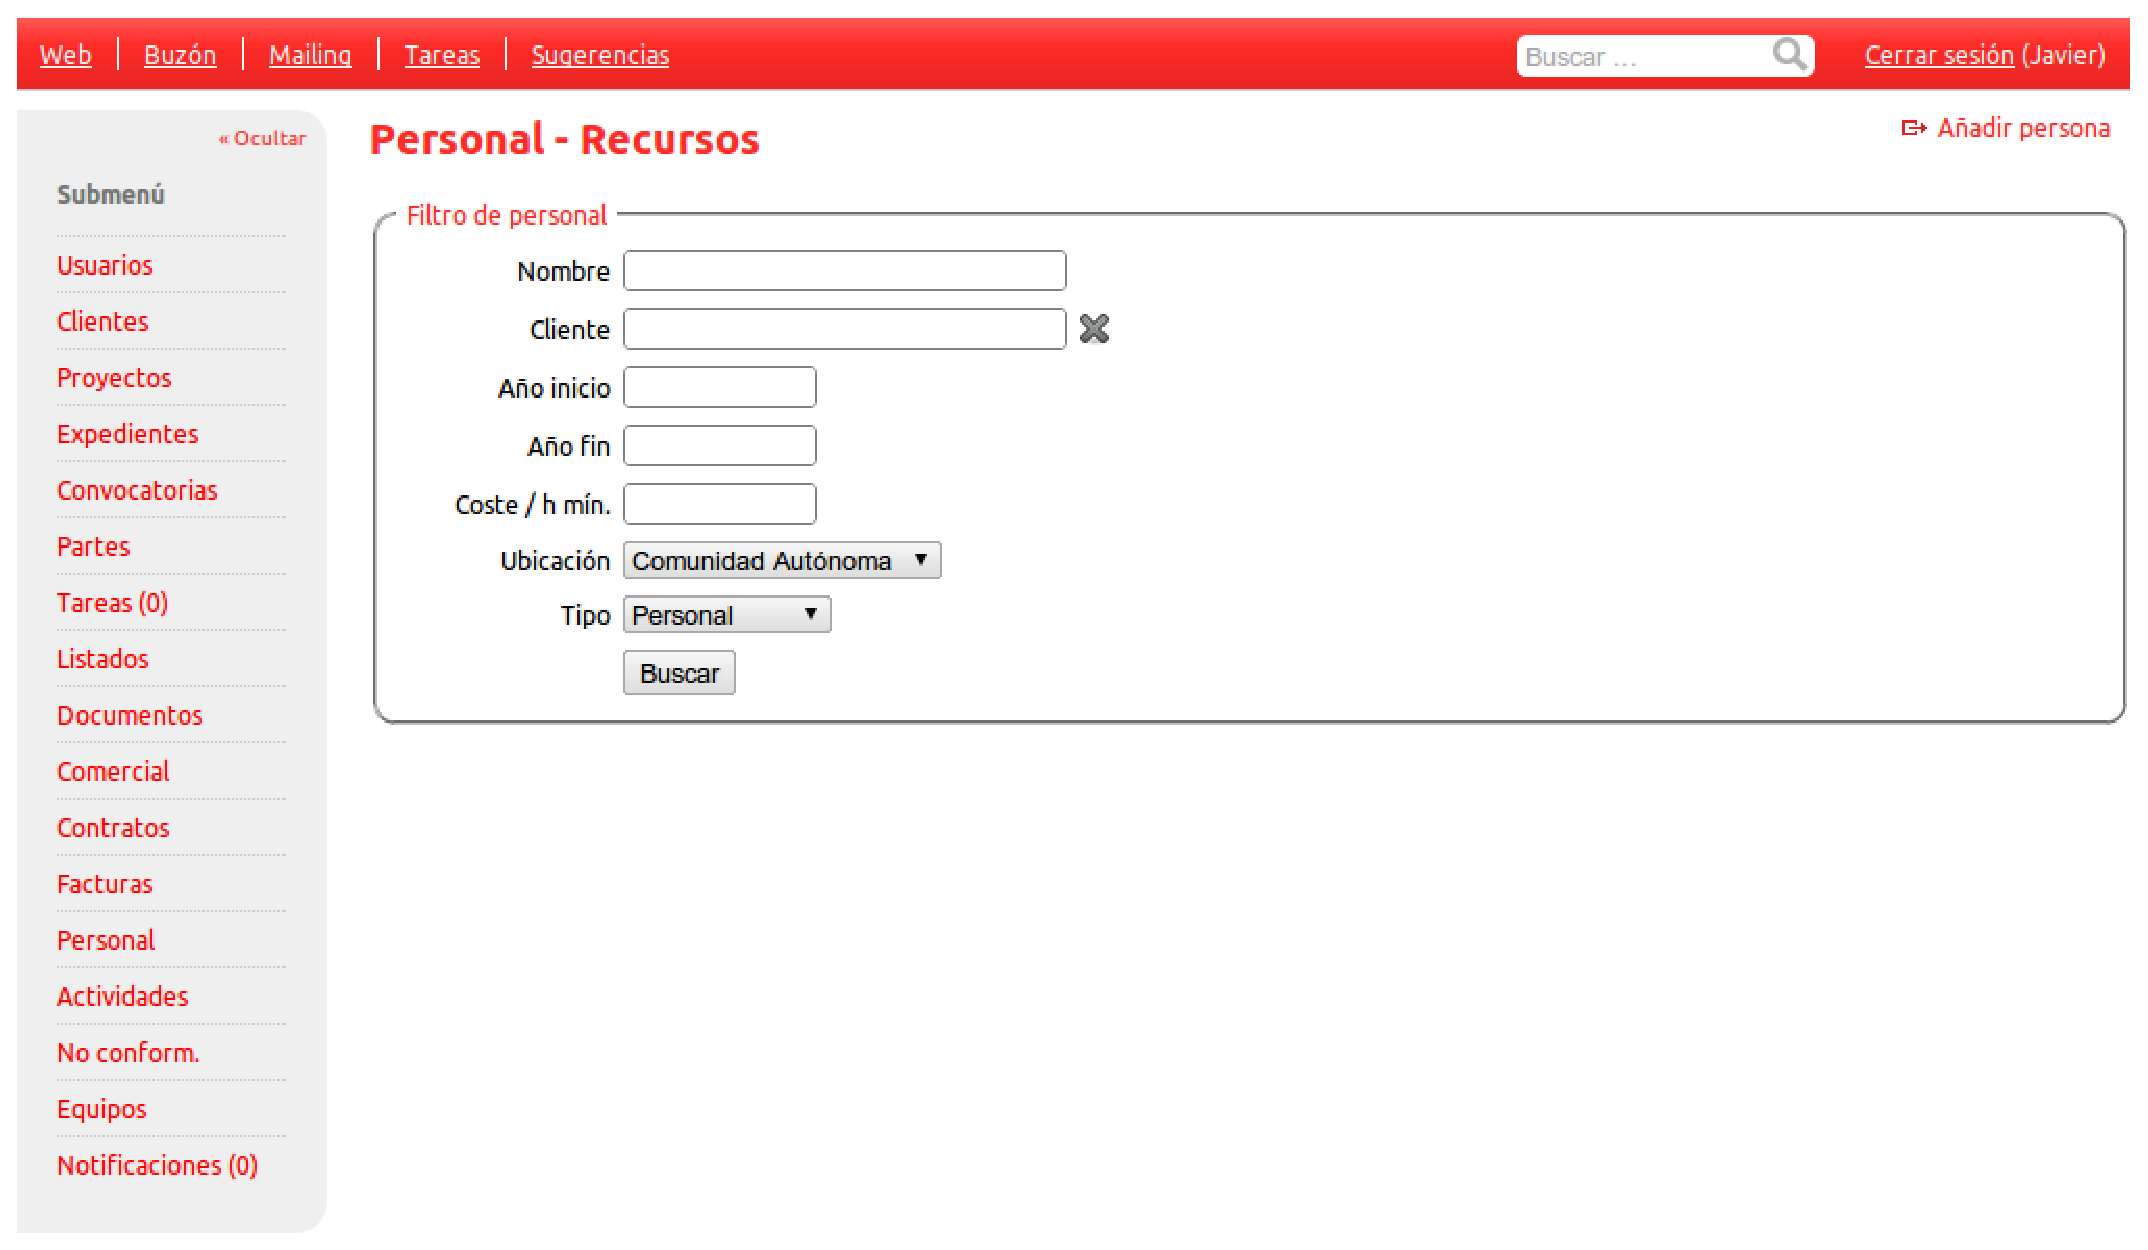
\epsfig{file=imagenes/manual/filtro_personal.eps,width=5.28in}
\caption{Filtro de personal.}
\label{fig:filtro_personal}
\end{figure}

Sin embargo, en general, solo queremos localizar un empleado concreto o
empleados de un mismo cliente, por lo que podemos hacer uso de cualquiera
combinación de los campos del filtro:

\begin{description}
 \item[Nombre] La búsqueda por nombre nos devuelve cualquier empleado cuyo
nombre contenga la cadena introducida.
 \item[Cliente] La búsqueda por cliente es un poco más sofisticada: cuando
introducimos más de tres caracteres, se nos sugieren hasta 20 clientes que
pueden tener relación con la cadena introducida, ya sea por su nombre o
acrónimo (figura \ref{fig:sug_cliente}). Si seleccionamos una de esas
sugerencias, la aplicación deja de usar la cadena como referencia en favor del
identificador del cliente y nos devolverá únicamente los empleados de ese
cliente, al margen de que otros clientes también satisfagan la cadena
introducida.
  \begin{figure}
  \centering
  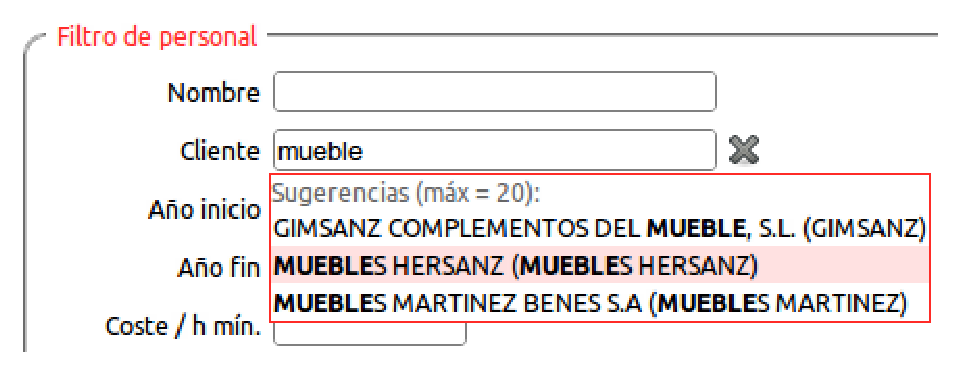
\epsfig{file=imagenes/manual/sug_cliente.eps,width=3.96in}
  \caption{Sugerencias de cliente.}
  \label{fig:sug_cliente}
  \end{figure}
 \item[Año inicio / Año fin] Si los empleados de una empresa llevan muchos años
trabajando, puede que no nos interese conocer los datos que se refieren a hace
más de 5 años, o puede que estemos buscando aquellos precisamente.
 \item[Coste por hora mínimo] Este apartado sirve para encontrar a los
empleados que ganan más de un determinado valor, lo que puede ser interesante a
la hora de planificar proyectos, implicando a trabajadores que ganan más para
obtener una subvención mayor.
 \item[Ubicación] Se refiere a la Comunidad Autónoma de procedencia del
empleado. Especialmente útil para localizar empleados de una de las sedes de
los clientes intercomunitarios.

\end{description}

\subsection{Creación de un nuevo empleado y de sus datos anuales}

Para crear un nuevo empleado, basta con hacer clic en el enlace que aparece en
la esquina superior derecha de cualquier página del módulo de \textbf{Personal}
(figura \ref{fig:aniadir_persona}).

\begin{figure}
\centering
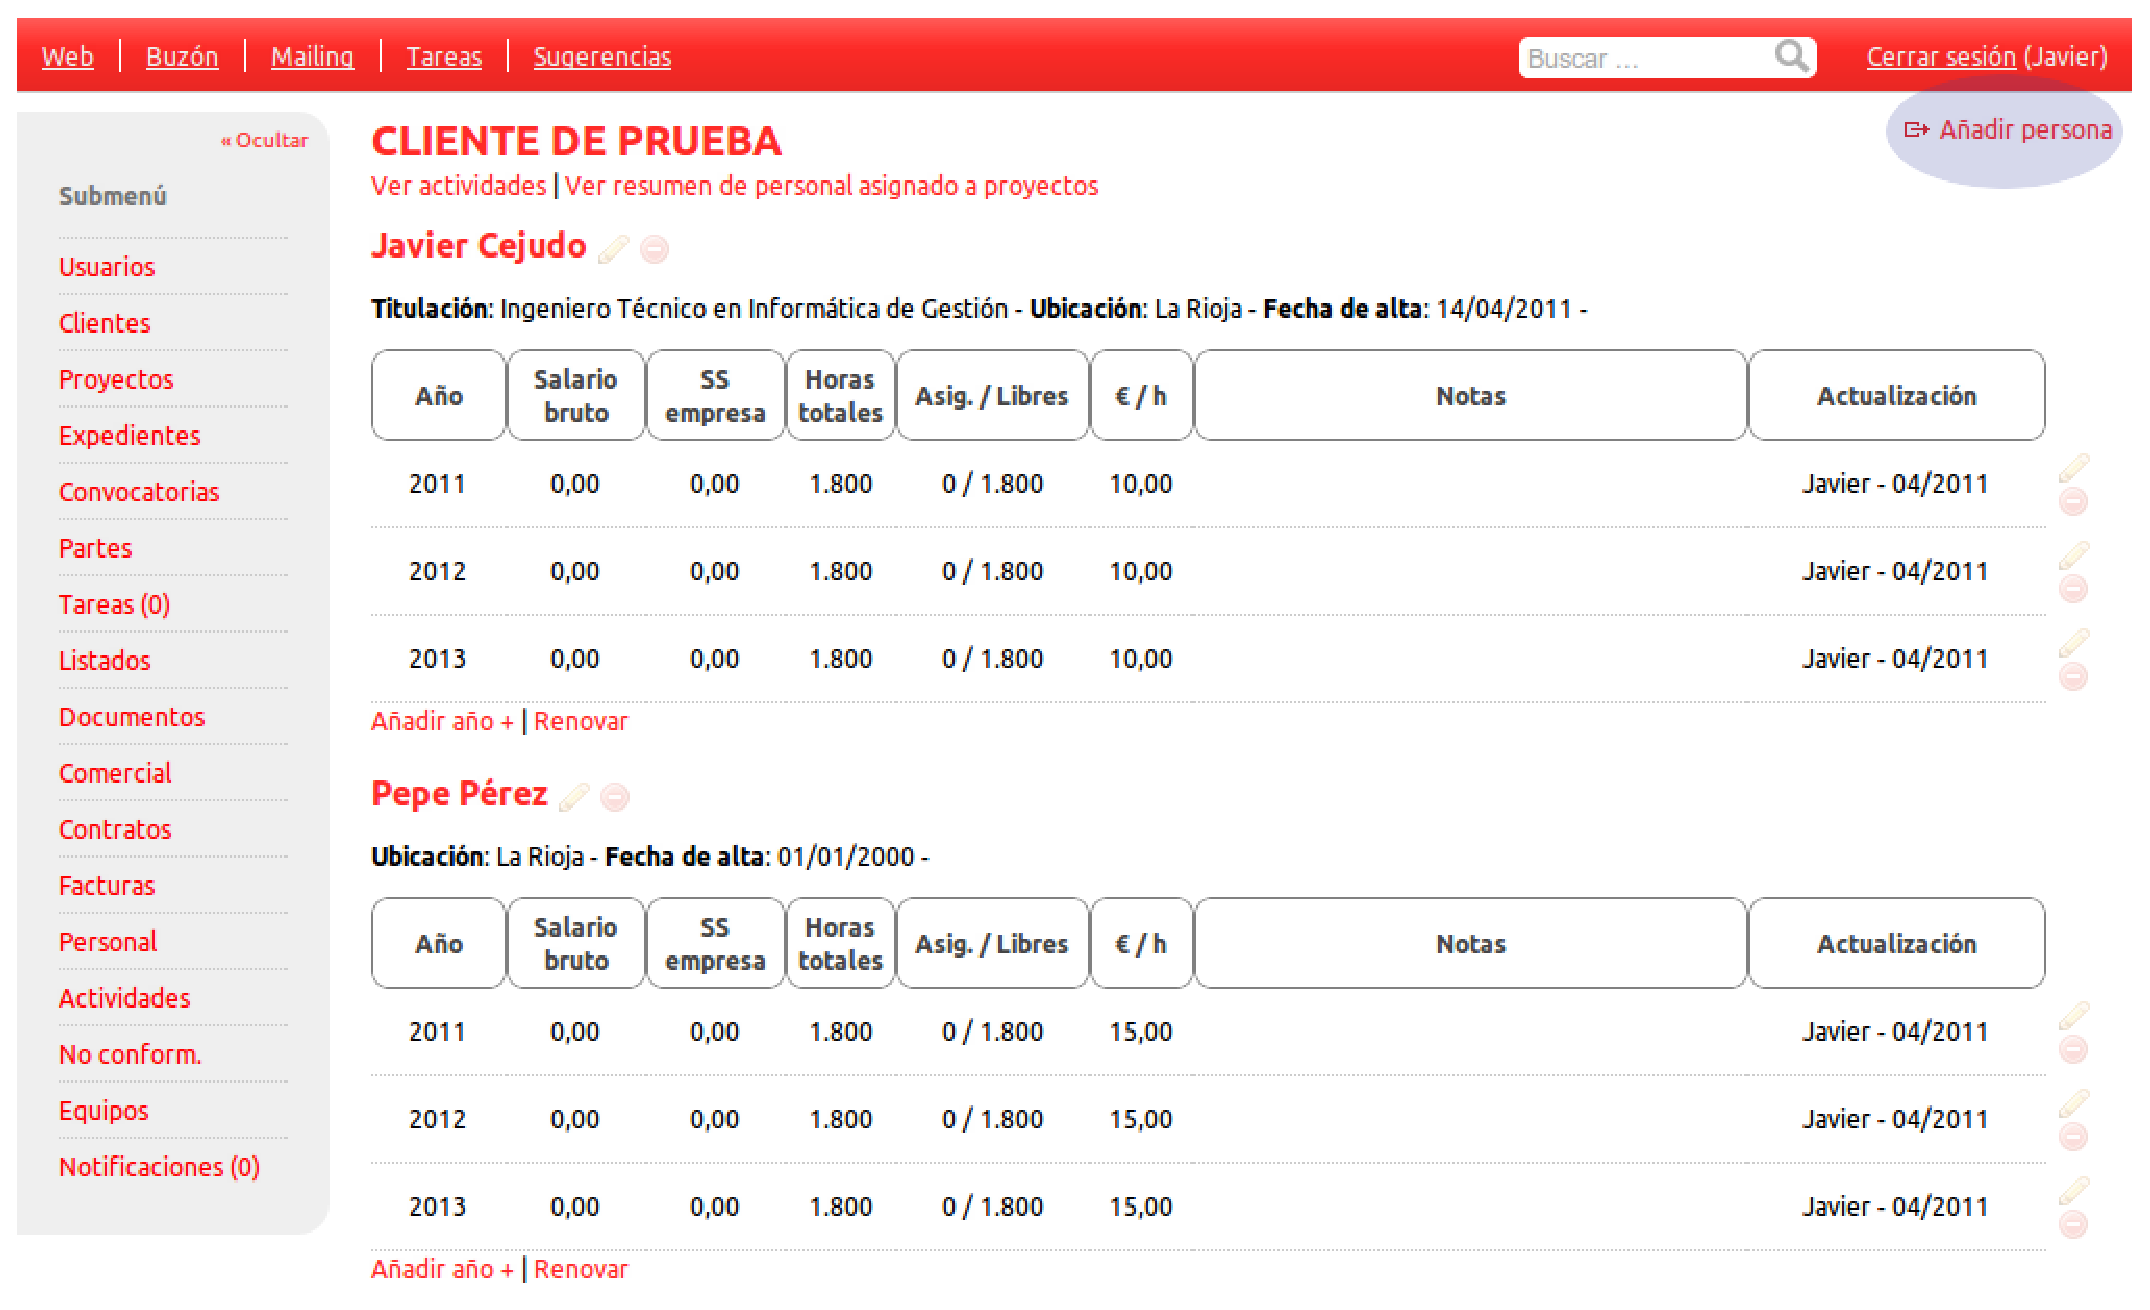
\epsfig{file=imagenes/manual/aniadir_persona.eps,width=5.28in}
\caption{Enlace para añadir personal.}
\label{fig:aniadir_persona}
\end{figure}

Una vez hemos pinchado en el enlace, nos aparecerá el formulario de la figura
\ref{fig:form_personal}, que debemos rellenar, al menos, con los datos
obligatorios: nombre y cliente. Cabe destacar que si hemos realizado una
búsqueda para un cliente concreto, el enlace a \textbf{Añadir persona} pasa la
información del cliente al formulario, por lo que simplemente añadiendo un
nombre, ya tendríamos un empleado nuevo. Siempre podemos modificar los datos
más adelante, como se indica en este mismo manual.

\begin{figure}
\centering
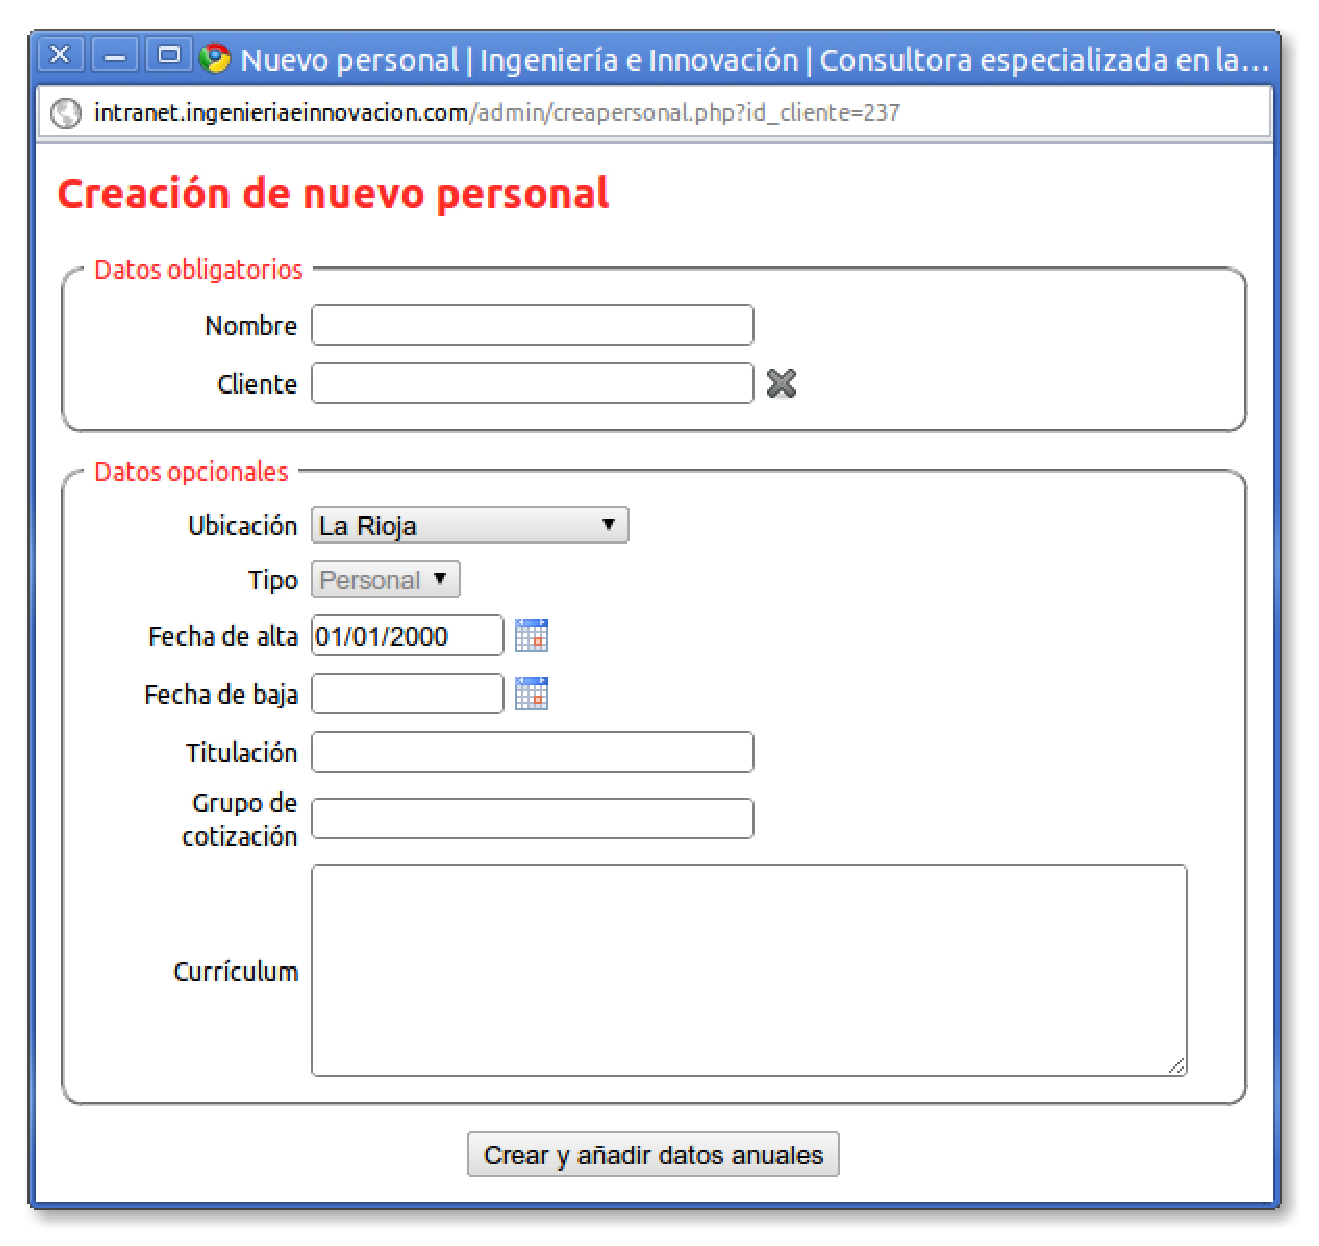
\epsfig{file=imagenes/manual/form_personal.eps,width=4in}
\caption{Creación de nuevo personal.}
\label{fig:form_personal}
\end{figure}

Una vez rellenado el formulario, hay que enviar los datos. Vemos que el enlace
para enviar el formulario dice \textbf{Crear y añadir datos anuales}. Esto se
debe a que un empleado sin datos anuales no es interesante para la aplicación,
ya que no podríamos imputarle horas. El formulario para los datos anuales se
puede ver en la figura \ref{fig:form_anuales}.

\begin{figure}
\centering
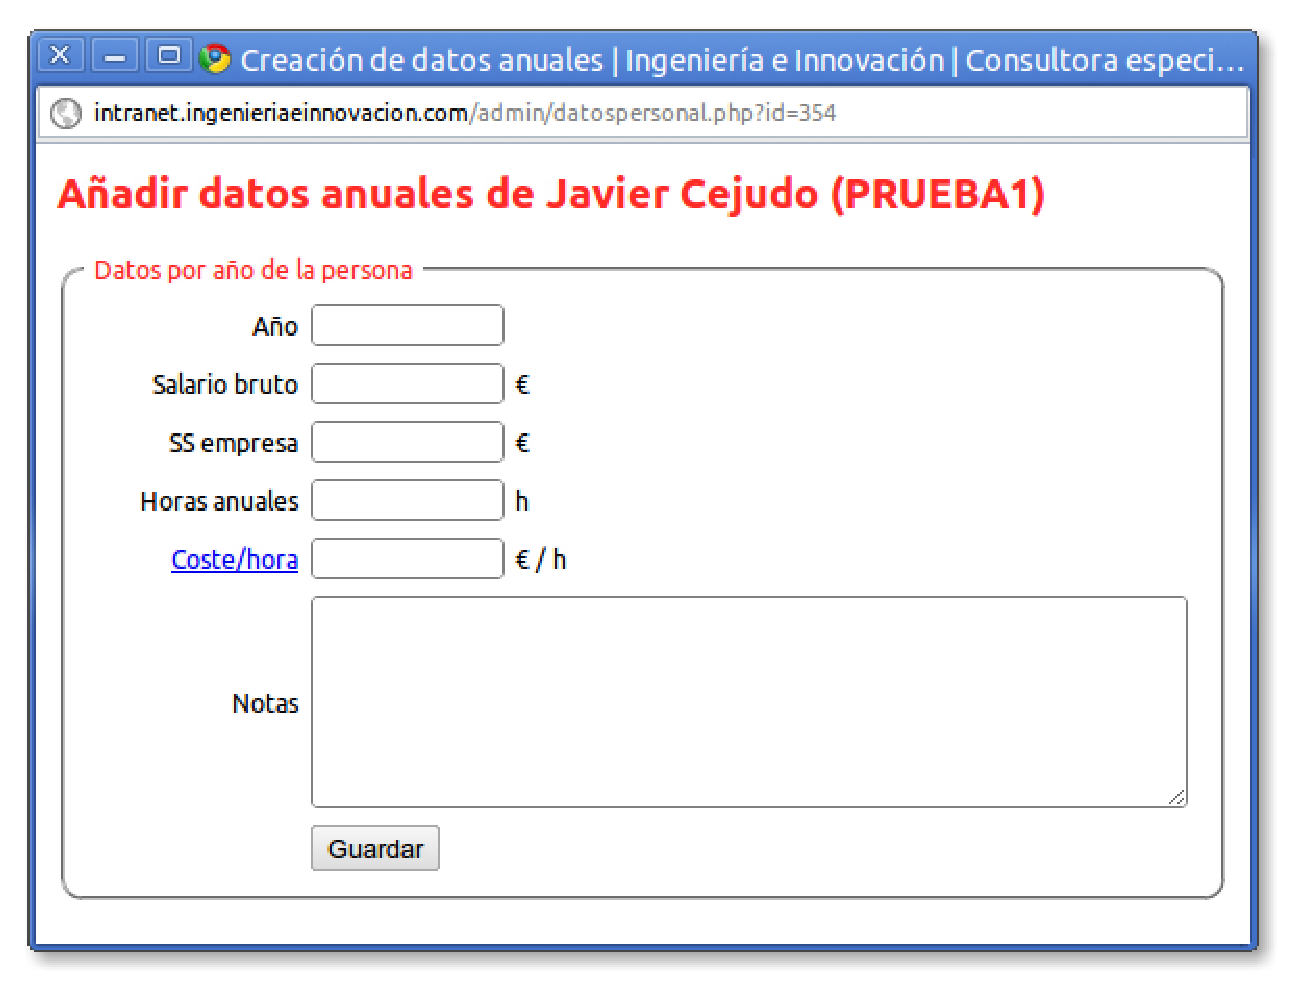
\epsfig{file=imagenes/manual/form_anuales.eps,width=4in}
\caption{Creación de datos anuales.}
\label{fig:form_anuales}
\end{figure}

Los datos obligatorios de este formulario son el \textbf{año} y el
\textbf{coste/hora}; sin embargo, si tenemos los datos acerca del salario
bruto, la Seguridad Social a cargo de la empresa y las horas anuales del
convenio, el coste/hora se calculará automáticamente.

Para añadir más datos anuales, podemos hacer clic en los enlaces que aparecen
debajo de la tabla de datos anuales de cada empleado (figura
\ref{fig:aniadir_anuales}).

\begin{figure}
\centering
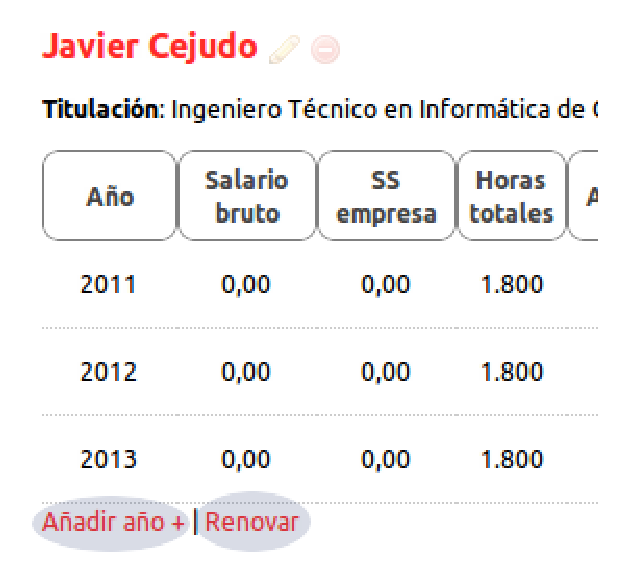
\epsfig{file=imagenes/manual/aniadir_anuales.eps,width=3in}
\caption{Enlaces para añadir datos anuales.}
\label{fig:aniadir_anuales}
\end{figure}

\begin{description}
 \item [Añadir año +] Este enlace nos lleva al mismo formulario de la figura
\ref{fig:form_anuales}, pero nos sugiere un valor de horas anuales basándose en
años anteriores o en datos de otros empleados.
 \item [Renovar] Este enlace añade automáticamente el año inmediatamente
posterior al más reciente, tomando como referencia sus datos (horas del
convenio, salario...).
\end{description}

\subsection{Modificación de un empleado y de sus datos anuales}

La necesidad de modificar un empleado es bastante común, ya sea para añadir
datos que se dejaron sin completar en la creación o para actualizar o corregir
datos erróneos. Esta acción se puede llevar a cabo fácilmente haciendo clic en
el icono que representa un lapicero, y que se puede encontrar al lado del
nombre del empleado (figura \ref{fig:mod_persona}).

\begin{figure}
\centering
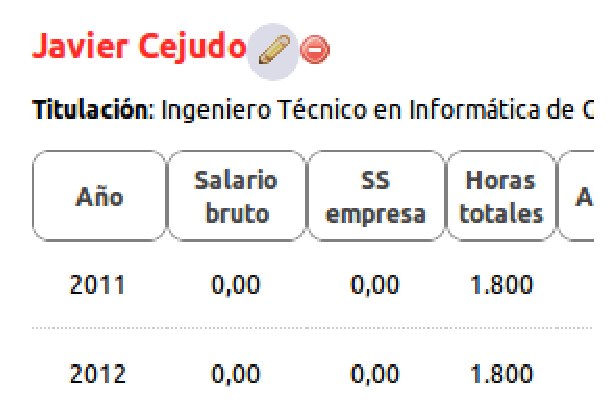
\epsfig{file=imagenes/manual/mod_persona.eps,width=3in}
\caption{Enlace para modificar los datos de un empleado.}
\label{fig:mod_persona}
\end{figure}

Entonces, nos aparecerá un formulario con los datos actuales del empleado
(figura \ref{fig:form_mod_persona}), que podemos modificar con la nueva
información de la que disponemos. Cabe destacar que no puede modificarse el
cliente al que pertenece el empleado debido a que podría tener horas imputadas
con el cliente actual y crearse inconsistencias.

\begin{figure}
\centering
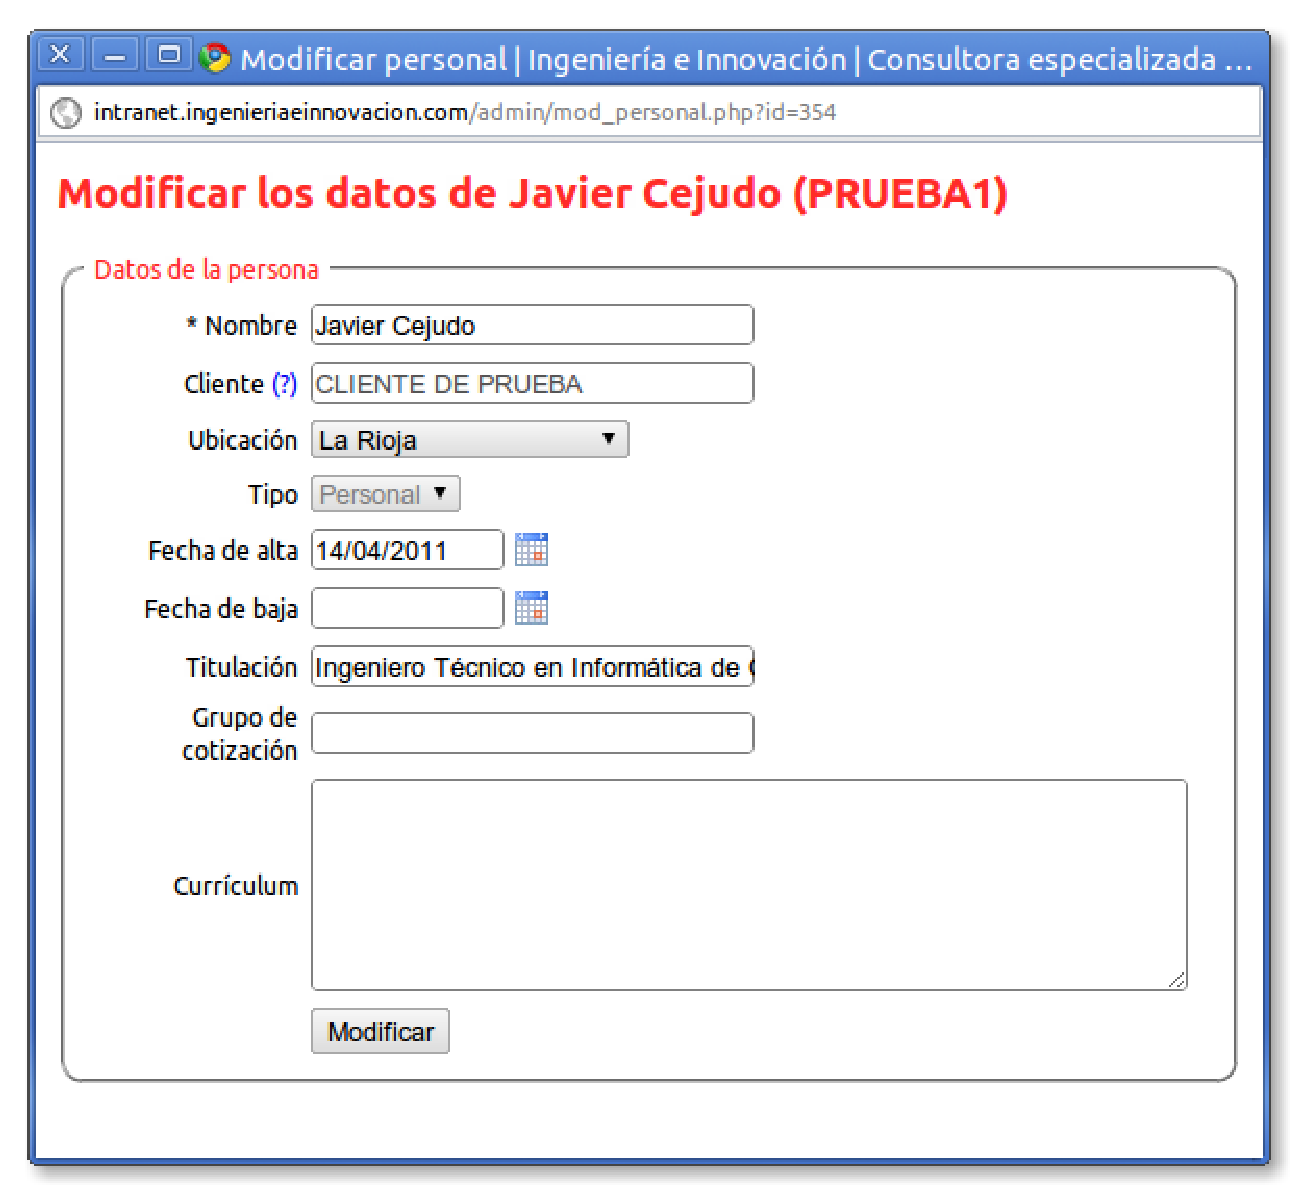
\epsfig{file=imagenes/manual/form_mod_persona.eps,width=5.28in}
\caption{Formulario de modificación de empleados.}
\label{fig:form_mod_persona}
\end{figure}

Los datos anuales pueden modificarse desde los enlaces de la parte derecha de
la tabla de datos anuales. El icono para modificar elementos en la aplicación es
siempre un lapicero (figura \ref{fig:mod_anuales}).

\begin{figure}
\centering
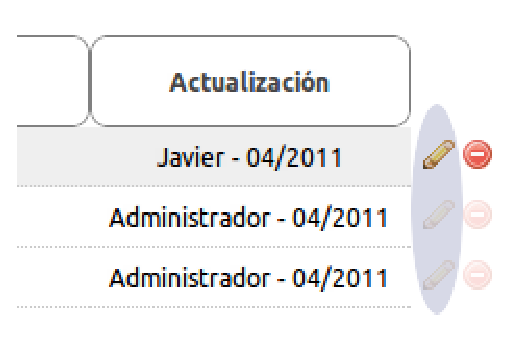
\epsfig{file=imagenes/manual/mod_anuales.eps,width=2.28in}
\caption{Enlace para modificar datos anuales.}
\label{fig:mod_anuales}
\end{figure}

En el formulario de modificación de datos anuales (figura
\ref{fig:form_mod_anuales}), podemos modificar cualquier valor excepto el año,
debido a que una modificación de ese tipo lleva implícita la desaparición de un
año al que se pueden haber imputado horas. 

\begin{figure}
\centering
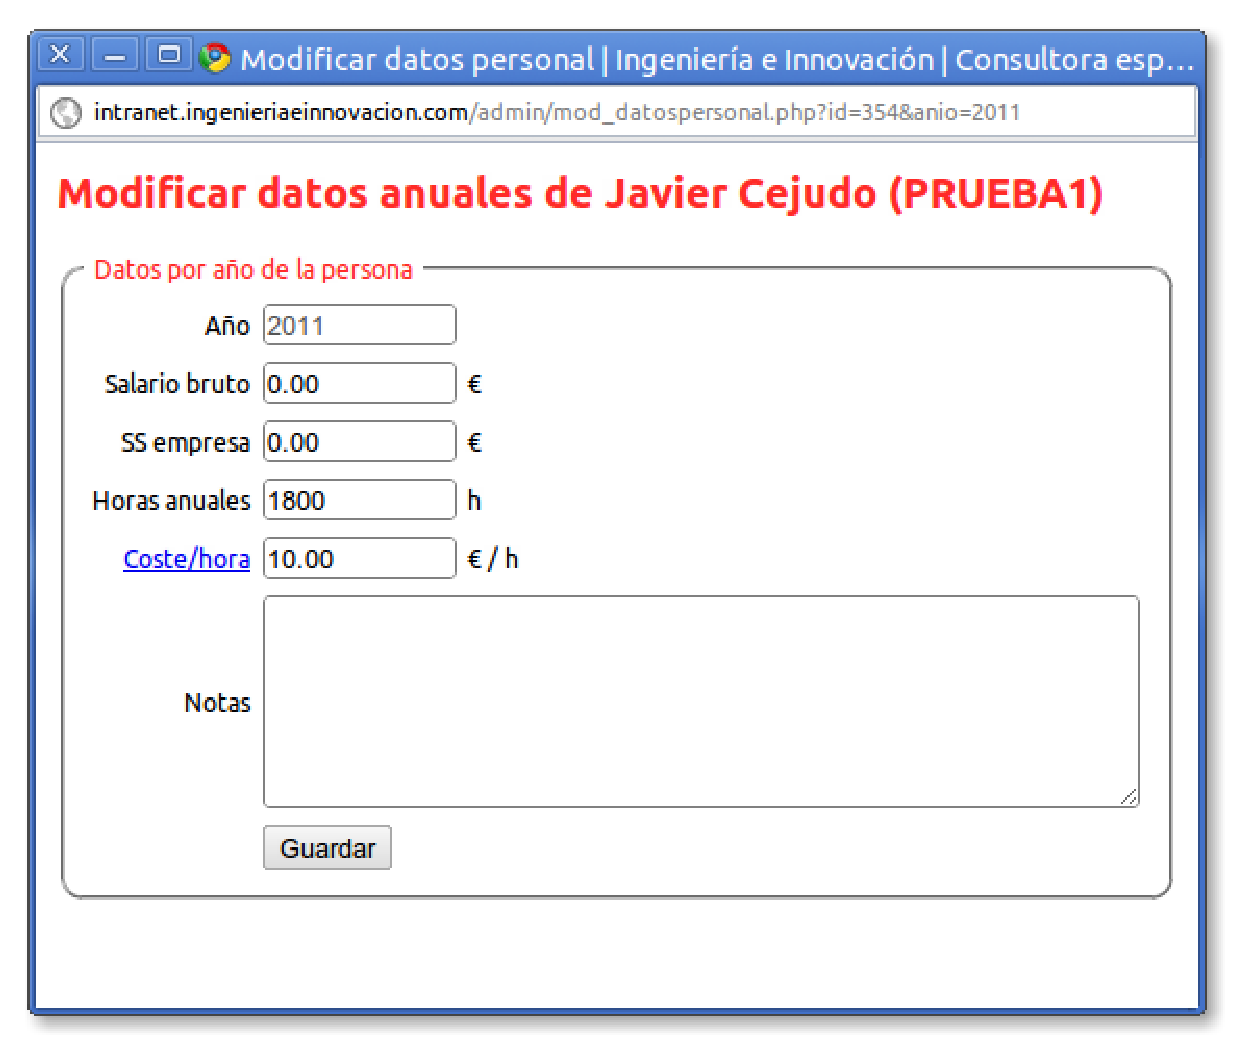
\epsfig{file=imagenes/manual/form_mod_anuales.eps,width=3.64in}
\caption{Formulario de modificación de empleados.}
\label{fig:form_mod_anuales}
\end{figure}

\subsection{Eliminación de un empleado y de sus datos anuales}

La eliminación de empleados y de sus datos anuales son acciones de alto riesgo.
Cualquiera de estas acciones borraría a su vez las decenas sino cientos de
datos referentes a horas imputadas del empleado. Es por ello que estas acciones
solamente pueden ser llevadas a cabo por el usuario Administrador. La
disposición de los iconos es totalmente análoga a la de modificación de
personal (figuras \ref{fig:bor_persona} y \ref{fig:bor_anuales}). En cualquier
caso, se nos pedirá confirmar la acción.

\begin{figure}
\centering
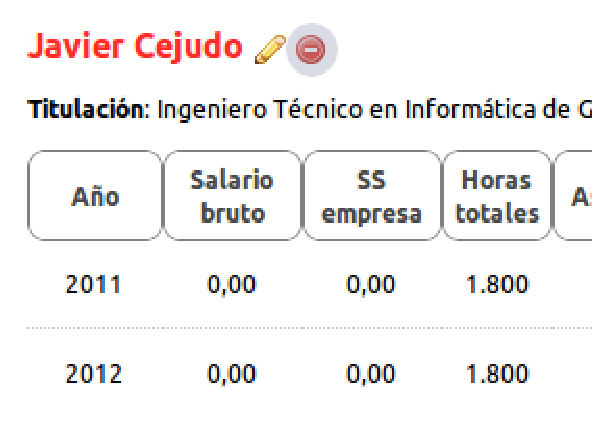
\epsfig{file=imagenes/manual/bor_persona.eps,width=3in}
\caption{Enlace para borrar los datos de un empleado.}
\label{fig:bor_persona}
\end{figure}

\begin{figure}
\centering
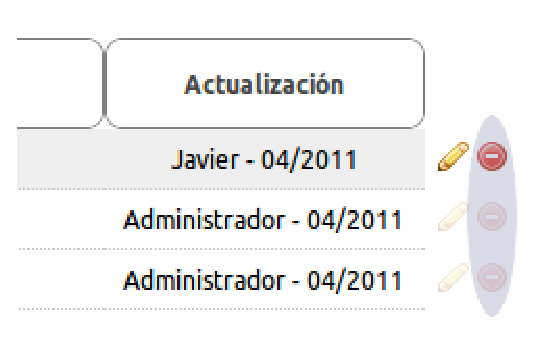
\epsfig{file=imagenes/manual/bor_anuales.eps,width=2.28in}
\caption{Enlace para borrar datos anuales.}
\label{fig:bor_anuales}
\end{figure}


% % % % % % % % % % % % % % % % % % % % % % % % % % % % % % % % % % % % 
% % % % % % % % % % % % % % % % % % % % % % % % % % % % % % % % % % % % 

% % % % % % % % % % % % % % % % % % % % % % % % % % % % % % % % % % % % 
% % % % % % % % % % % % % % % % % % % % % % % % % % % % % % % % % % % % 

% % % % % % % % % % % % % % % % % % % % % % % % % % % % % % % % % % % % 
% % % % % % % % % % % % % % % % % % % % % % % % % % % % % % % % % % % % 


\section{Gestión de actividades}
\label{sec:manual_actividades}

Para una gestión integral de las actividades, debemos ser capaces de crear
nuevas actividades, modificar actividades existentes y borrar actividades. Las
actividades deben formar parte de un proyecto y solo de un proyecto.

Para comenzar a gestionar actividades, lo primero que debemos hacer es
seleccionar la entrada del menú con el nombre \textbf{Actividades}, como se ve
en la figura \ref{fig:inicio_act}.

\begin{figure}
\centering
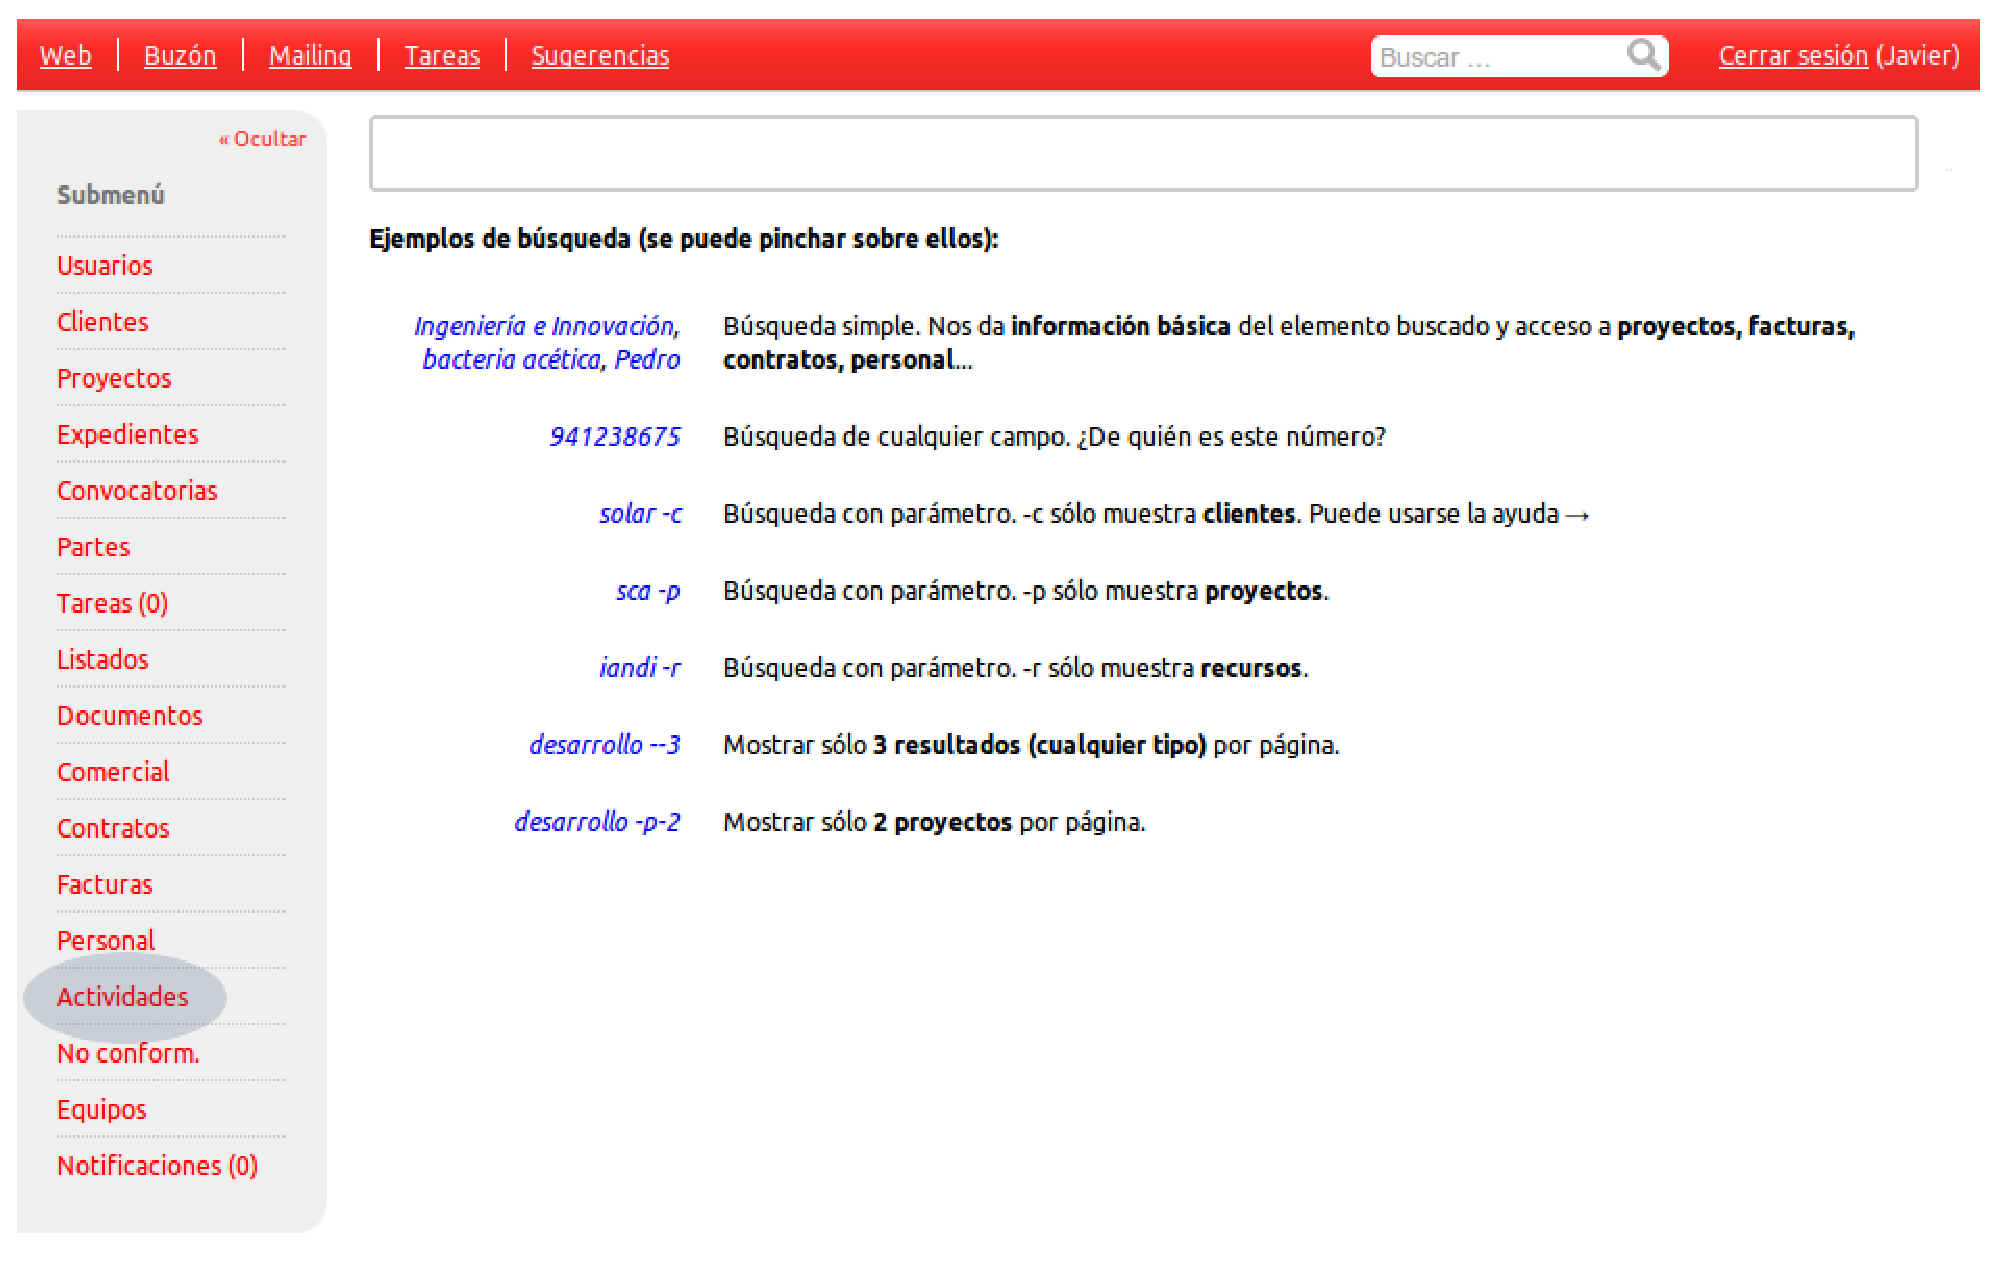
\epsfig{file=imagenes/manual/inicio_act.eps,width=5.28in}
\caption{Enlace al módulo de actividades en el menú.}
\label{fig:inicio_act}
\end{figure}

\subsection{Búsqueda de proyectos/actividades}
\label{sec:manual_busqueda_actividades}

Lo primero que nos encontramos es un buscador de actividades (figura
\ref{fig:filtro_act}), que funciona más propiamente como un filtro: esto
quiere decir que si no introducimos ningún valor y pulsamos \textbf{Buscar}, se
nos mostrarán todas las actividades de todos los proyectos.

\begin{figure}
\centering
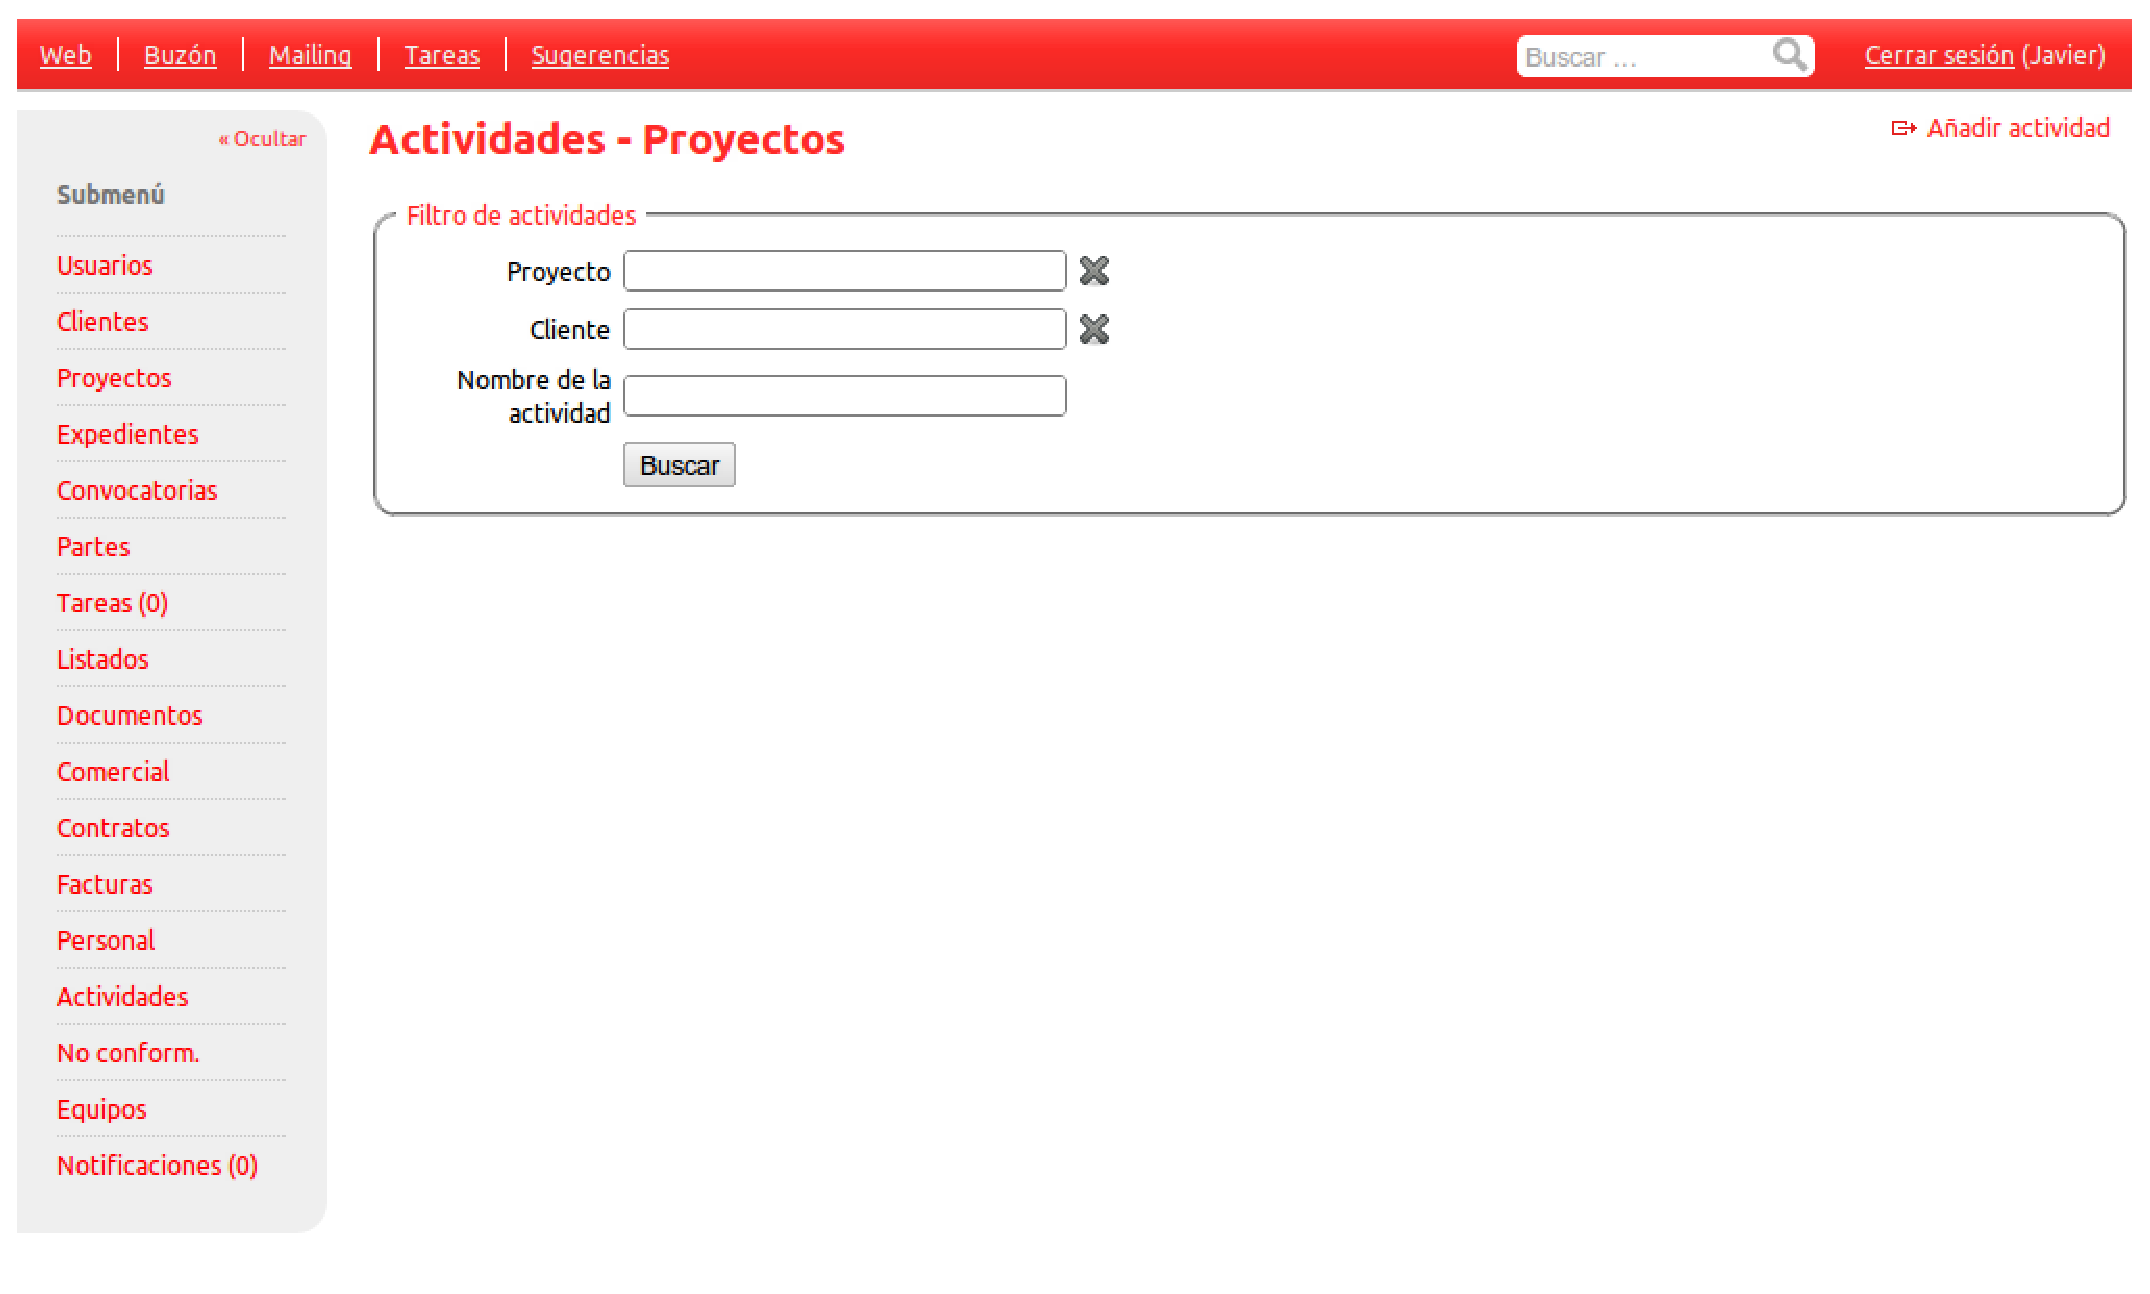
\epsfig{file=imagenes/manual/filtro_act.eps,width=5.28in}
\caption{Filtro de actividades.}
\label{fig:filtro_act}
\end{figure}

Sin embargo, en general, solo queremos localizar una actividad concreta o
todas las actividades de un mismo proyecto, por lo que podemos hacer uso de
cualquiera combinación de los campos del filtro:

\begin{description}
 \item[Proyecto] La búsqueda por cliente es más o menos sofisticada: cuando
introducimos más de tres caracteres, se nos sugieren hasta 20 proyectos que
pueden tener relación con la cadena introducida, ya sea por su nombre o
acrónimo (figura \ref{fig:sug_proyecto}) o por el nombre o acrónimo del cliente.
Si seleccionamos una de esas sugerencias, la aplicación deja de usar la cadena
como referencia en favor del identificador del proyecto y nos devolverá
únicamente los proyectos y las actividades de ese cliente, al margen de que
otros proyectos también satisfagan la cadena introducida.
  \begin{figure}
  \centering
  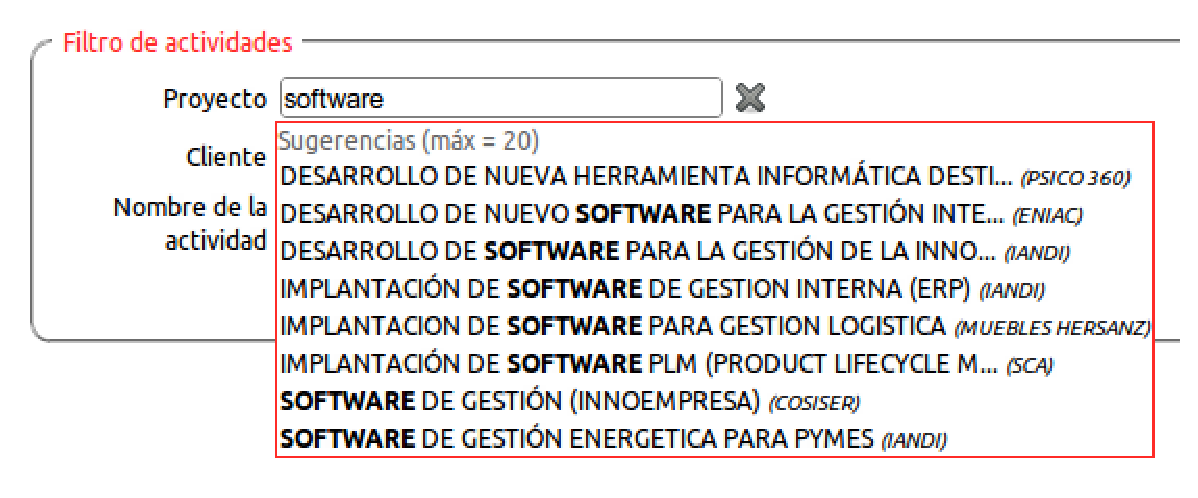
\epsfig{file=imagenes/manual/sug_proyecto.eps,width=3.88in}
  \caption{Sugerencias de proyecto.}
  \label{fig:sug_proyecto}
  \end{figure}
 \item[Cliente] La búsqueda por cliente funciona exactamente igual que en el
filtro de personal (figura \ref{fig:sug_cliente}).
 \item[Nombre] La búsqueda por nombre nos devuelve cualquier actividad cuyo
nombre contenga la cadena introducida.

\end{description}

\subsection{Creación de una nueva actividad}

Para crear una nueva actividad, basta con hacer clic en el enlace que aparece en
la esquina superior derecha de cualquier página del módulo de
\textbf{Actividades} o bien al final de la lista de actividades de cada
proyecto (figura \ref{fig:aniadir_actividad}).

\begin{figure}
\centering
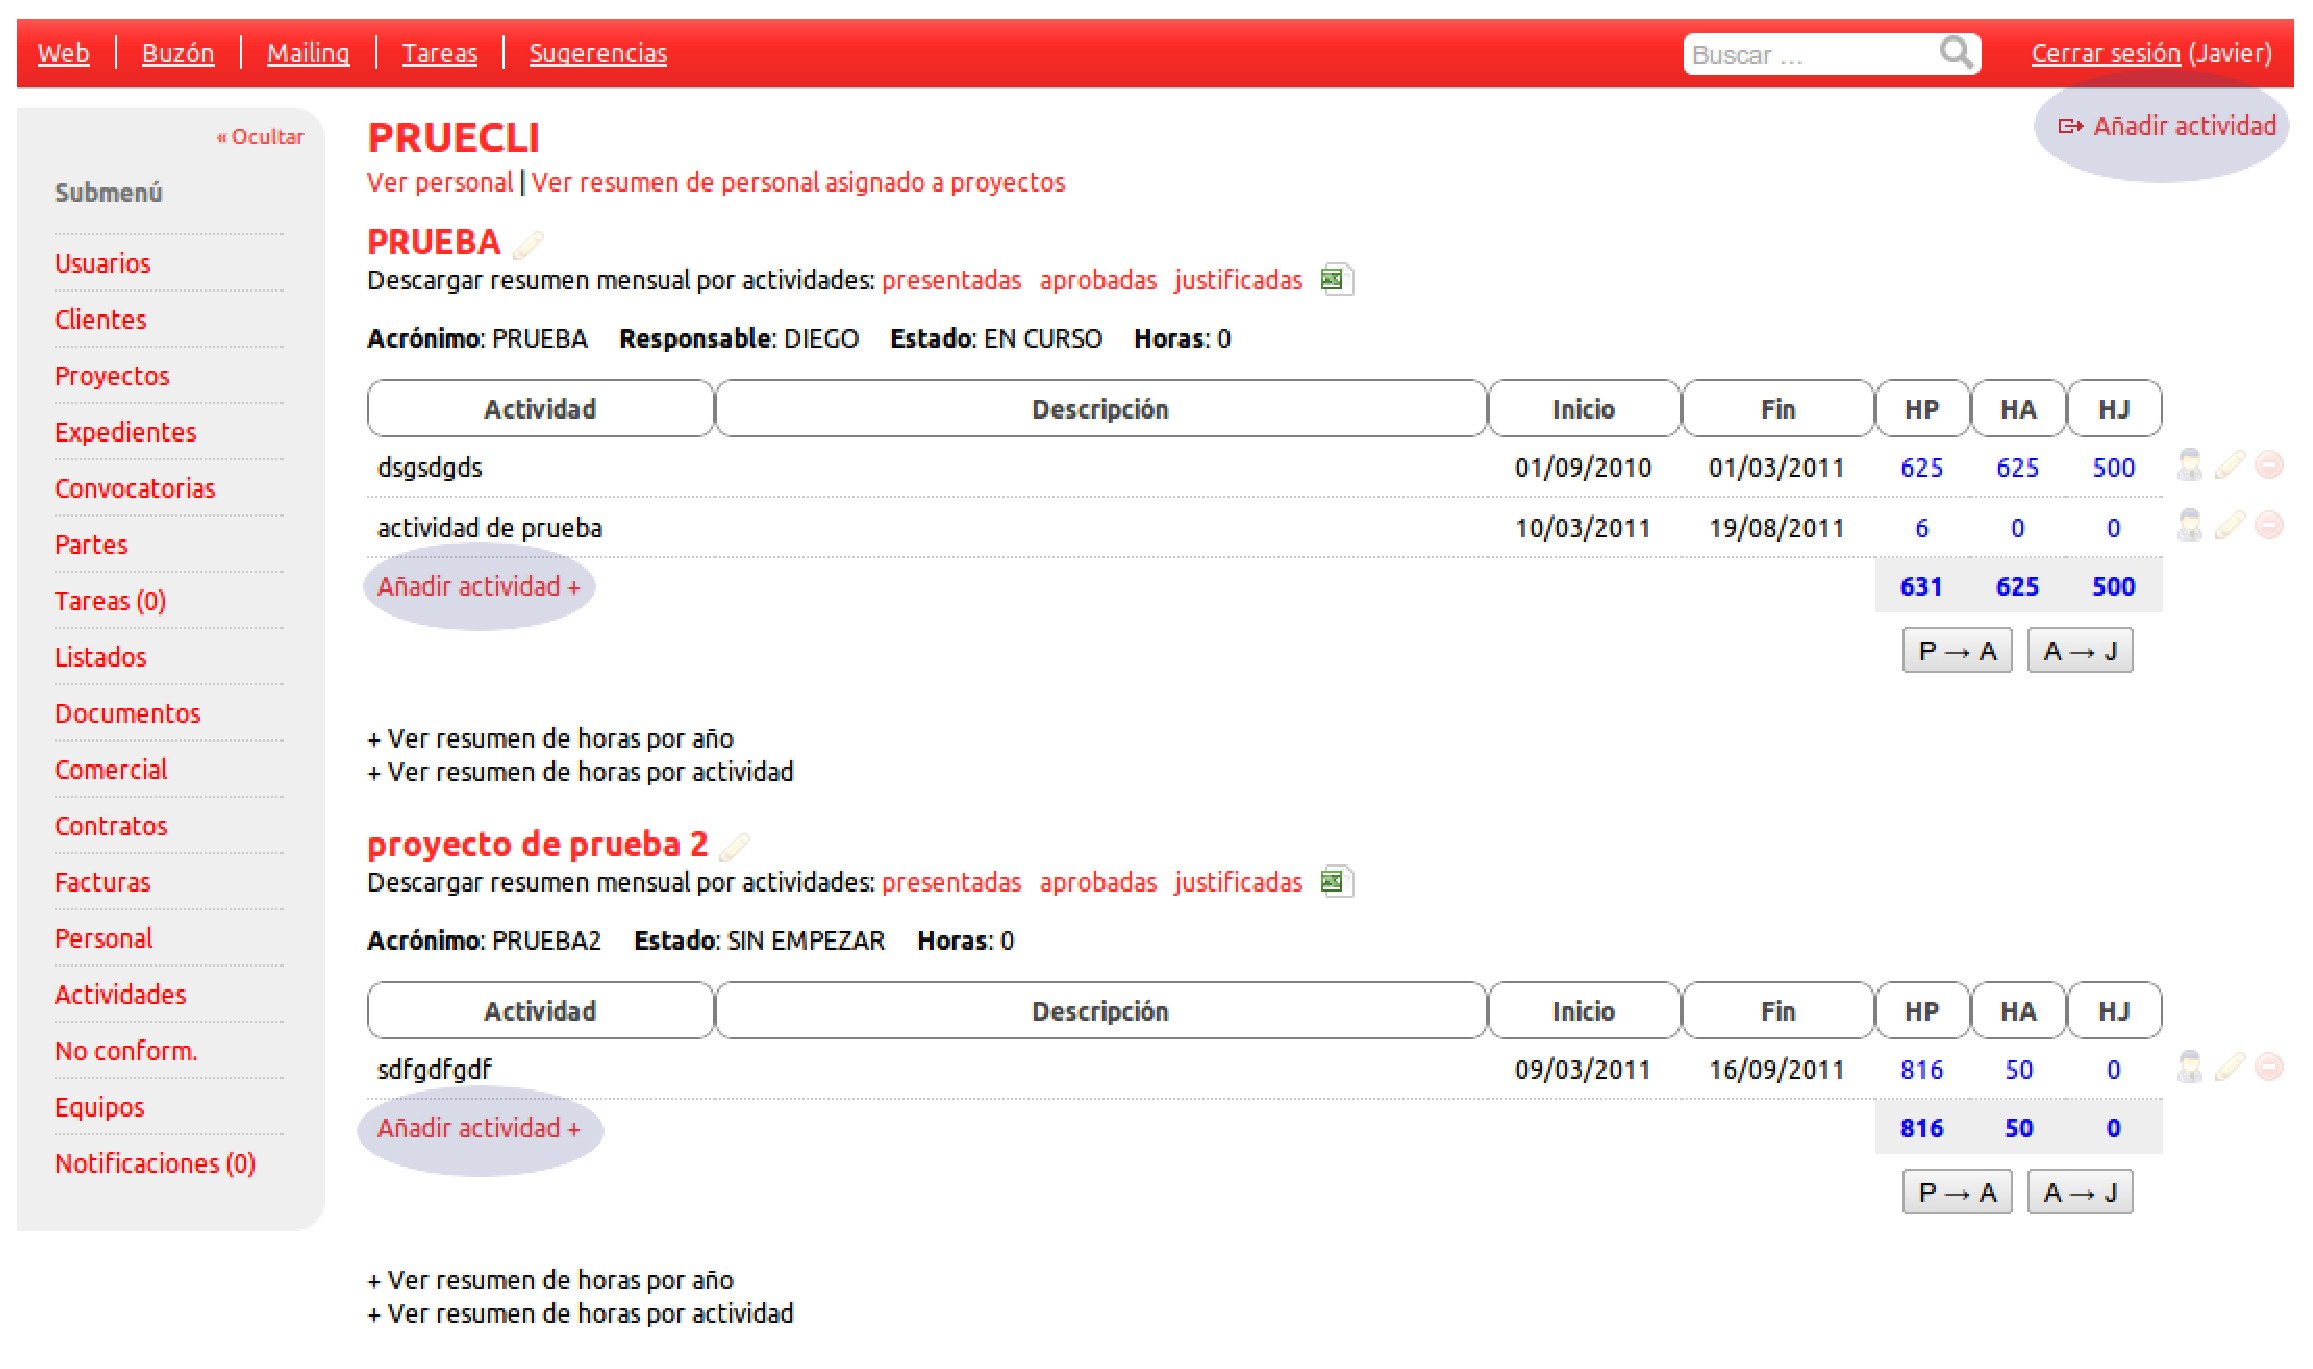
\epsfig{file=imagenes/manual/aniadir_actividad.eps,width=5.28in}
\caption{Enlaces para añadir actividades.}
\label{fig:aniadir_actividad}
\end{figure}

Una vez hemos pinchado en el enlace, nos aparecerá el formulario de la figura
\ref{fig:form_actividad}, que debemos rellenar, al menos, con los datos
obligatorios: proyecto, nombre, fecha de inicio y fecha de fin. Cabe destacar
que si hemos realizado una búsqueda para un proyecto concreto o si pinchamos el
enlace bajo la lista de actividades de un proyecto, el campo proyecto
aparecerá rellenado.

\begin{figure}
\centering
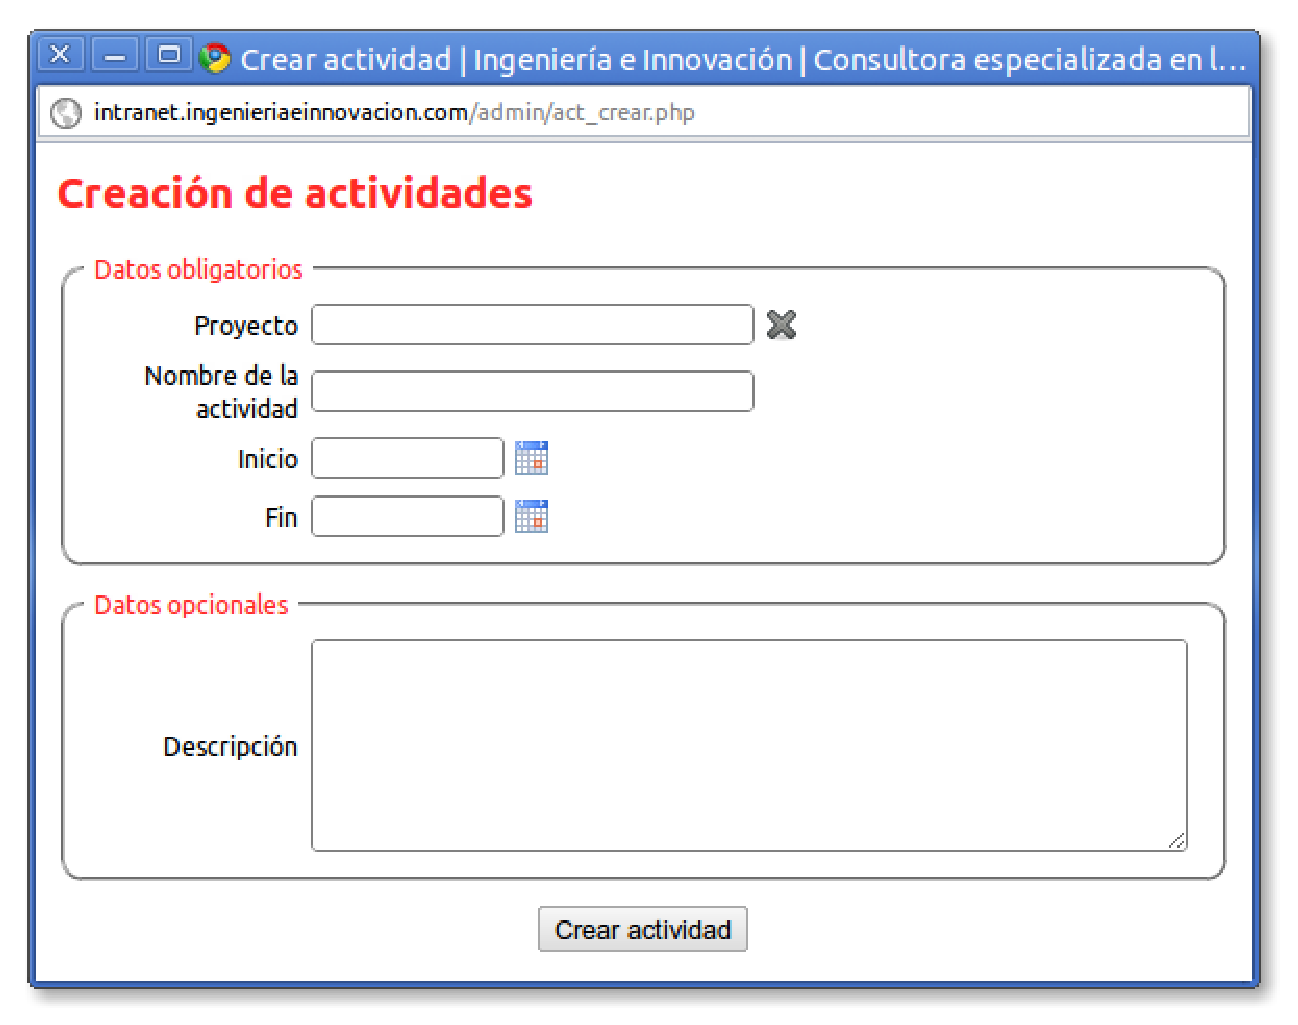
\epsfig{file=imagenes/manual/form_actividad.eps,width=4.21in}
\caption{Creación de nueva actividad.}
\label{fig:form_actividad}
\end{figure}


\subsection{Modificación de una actividad}

La necesidad de modificar una actividad es relativamente común, a pesar de que
la mayoría de los proyectos están plenamente planificados desde el inicio. Las
principales modificaciones se deben a desfases temporales en la ejecución de
proyecto. Esta acción se puede llevar a cabo fácilmente haciendo clic en el
icono que representa un lapicero, y que se puede encontrar en la parte de la
derecha de la tabla de actividades de cada proyecto (figura
\ref{fig:mod_actividad}).

\begin{figure}
\centering
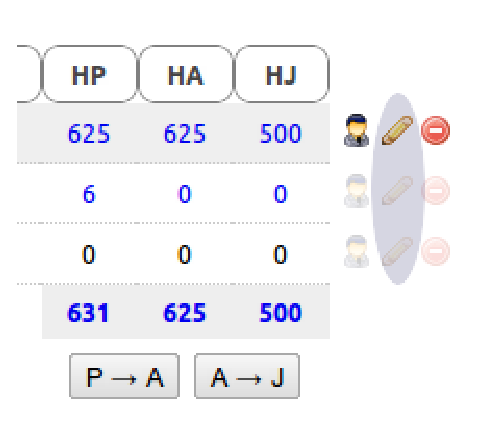
\epsfig{file=imagenes/manual/mod_actividad.eps,width=2.23in}
\caption{Enlace para modificar los datos de una actividad.}
\label{fig:mod_actividad}
\end{figure}

Entonces, nos aparecerá un formulario con los datos actuales de la actividad
(figura \ref{fig:form_mod_actividad}), que podemos modificar con la nueva
información de la que disponemos. Cabe destacar que no puede modificarse el
proyecto al que pertenece el empleado debido a que podría haber horas imputadas
con el proyecto actual y crearse inconsistencias.

\begin{figure}
\centering
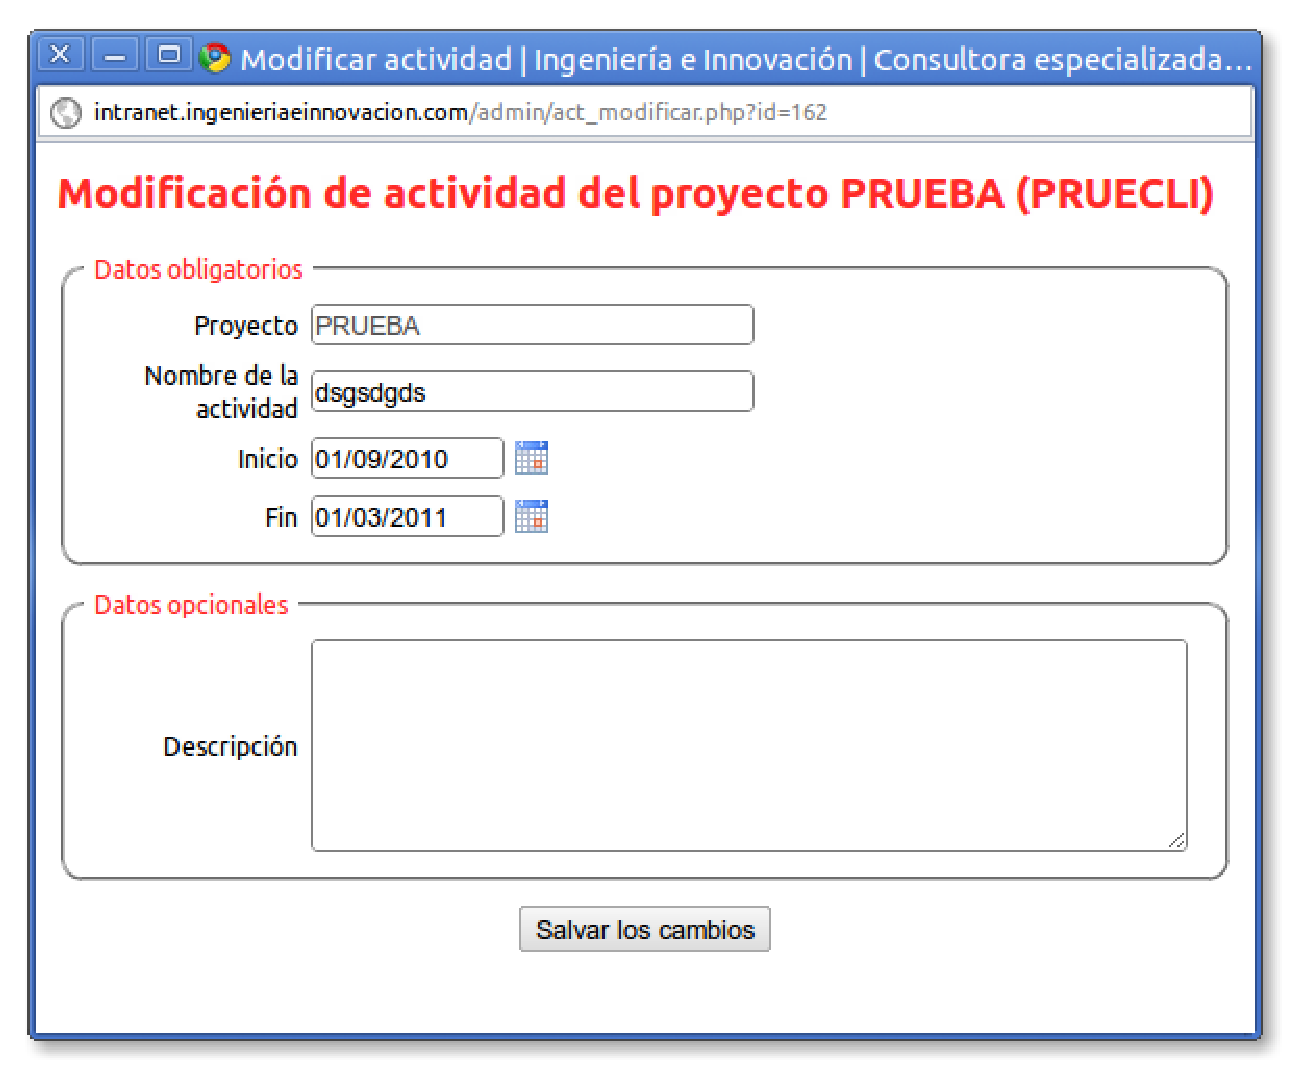
\epsfig{file=imagenes/manual/form_mod_actividad.eps,width=5.28in}
\caption{Formulario de modificación de empleados.}
\label{fig:form_mod_actividad}
\end{figure}
 
\subsection{Eliminación de una actividad}

La eliminación de actividades es una acción de alto riesgo, ya que con cada
actividad borrada, se pierden a su vez las decenas sino cientos de datos
referentes a horas imputadas. Es por ello que la eliminación de actividades
solamente puede ser llevada a cabo por el usuario Administrador. La
disposición de los iconos es totalmente análoga a la de modificación de
actividades (figura \ref{fig:bor_actividad}). En cualquier caso, se nos pedirá
confirmar la acción.

\begin{figure}
\centering
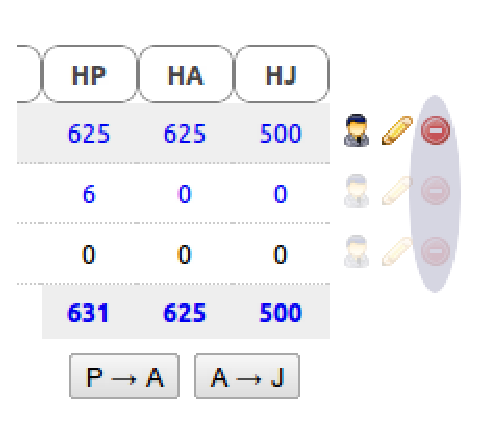
\epsfig{file=imagenes/manual/bor_actividad.eps,width=2.23in}
\caption{Enlace para borrar una actividad.}
\label{fig:bor_actividad}
\end{figure}

\section{Consulta de datos e informes}

La consulta de datos va a ser nuestra principal actividad como usuarios del
sistema, de modo que es importante que conozcamos todas las posibilidades que
este nos ofrece.

La consulta de personal y actividades se ha descrito en secciones
anteriores de este manual (\ref{sec:manual_personal},
\ref{sec:manual_actividades}), de manera que nos centraremos en la consulta de
horas asignadas, cuya gestión se describirá, a su vez, en la sección siguiente
(sección \ref{sec:manual_horas}).

La primera pregunta que nos debemos hacer es si estamos interesados en conocer
las horas asignadas a un recurso independientemente de los proyectos
involucrados, a un proyecto independientemente de los recursos asignados, o más
bien buscamos datos concretos sin \textit{variables libres}.

\subsection{Consulta de datos por personal}

La forma más rápida de conocer cuántas horas tiene asignadas un recurso en un
año concreto, es buscar a ese recurso como se explicó en la sección
\ref{sec:manual_busqueda_personal} y revisar sus horas asignadas anualmente
como se indica en la figura \ref{fig:horas_anuales}.

\begin{figure}
\centering
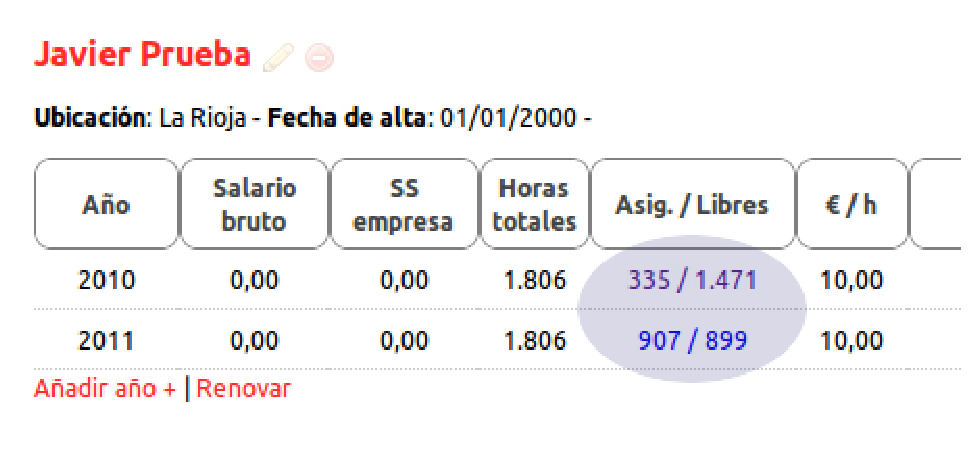
\epsfig{file=imagenes/manual/horas_anuales.eps,width=4.73in}
\caption{Horas asignadas a un empleado concreto en 2010 y 2011.}
\label{fig:horas_anuales}
\end{figure}

Cualquier valor de horas con la apariencia usual de los enlaces en la web es,
de hecho, un enlace a un informe desglosado por meses de esas horas. Así,
pinchando en el segundo de los valores señalados en la figura
\ref{fig:horas_anuales}, obtendremos el desglose de la figura
\ref{fig:desglose_horas}. En el filtro superior del desglose, que podemos
modificar a nuestro antojo, se aprecia que no hay seleccionado ningún proyecto,
y de hecho, vemos que están mezcladas las horas de dos proyectos: PRUEBA y
PRUEBA2.

\begin{figure}
\centering
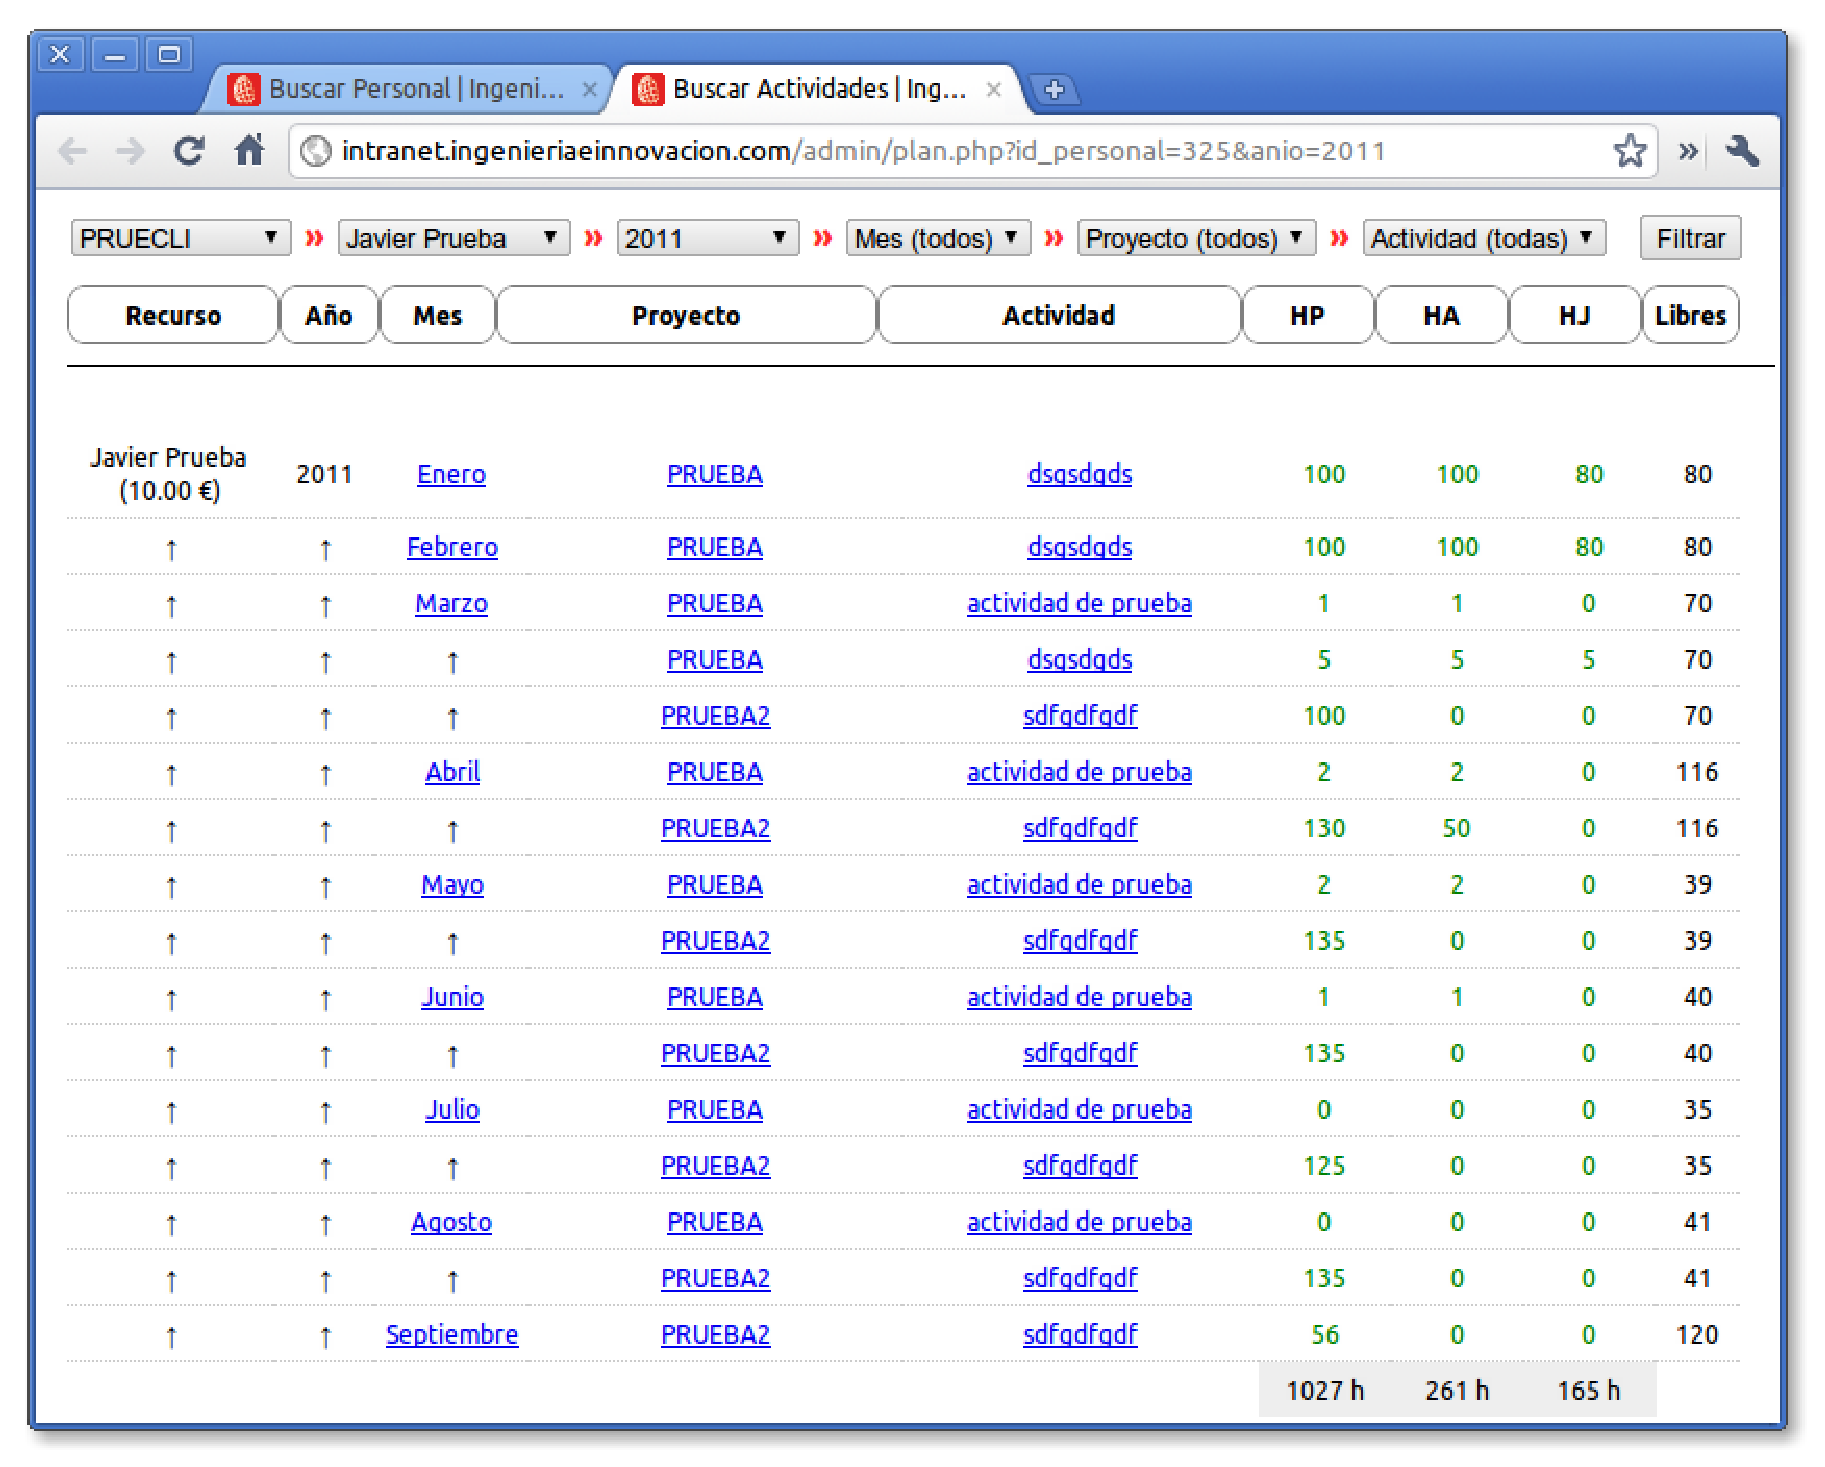
\epsfig{file=imagenes/manual/desglose_horas.eps,width=4.5in}
\caption{Desglose mensual de horas para un recurso concreto.}
\label{fig:desglose_horas}
\end{figure}

\subsection{Consulta de datos por proyecto}

La forma más rápida de conocer cuántas horas hay asignadas a un proyecto
concreto, es buscar ese proyecto como se explicó en la sección
\ref{sec:manual_busqueda_actividades}. En la página de cada proyecto,
encontraremos los siguientes informes:

\begin{description}
 \item [Desglose general por actividades (figura \ref{fig:consulta_horas_act})]
Este informe no identifica personal y su principal uso será la gestión de
actividades, más que la consulta de horas.
 \item [Resumen de horas por año (figura \ref{fig:horas_resumen_anio})] Muestra
el sumatorio de horas por año para cada empleado en las tres fases de la gestión
de los proyectos: presentación, aprobación y justificación.
 \item [Resumen de horas por actividad (figura
\ref{fig:horas_resumen_actividad})] Muestra el sumatorio de horas por actividad
para cada empleado en las tres fases de la gestión de los proyectos:
presentación, aprobación y justificación.
 
\end{description}

\begin{figure}
\centering
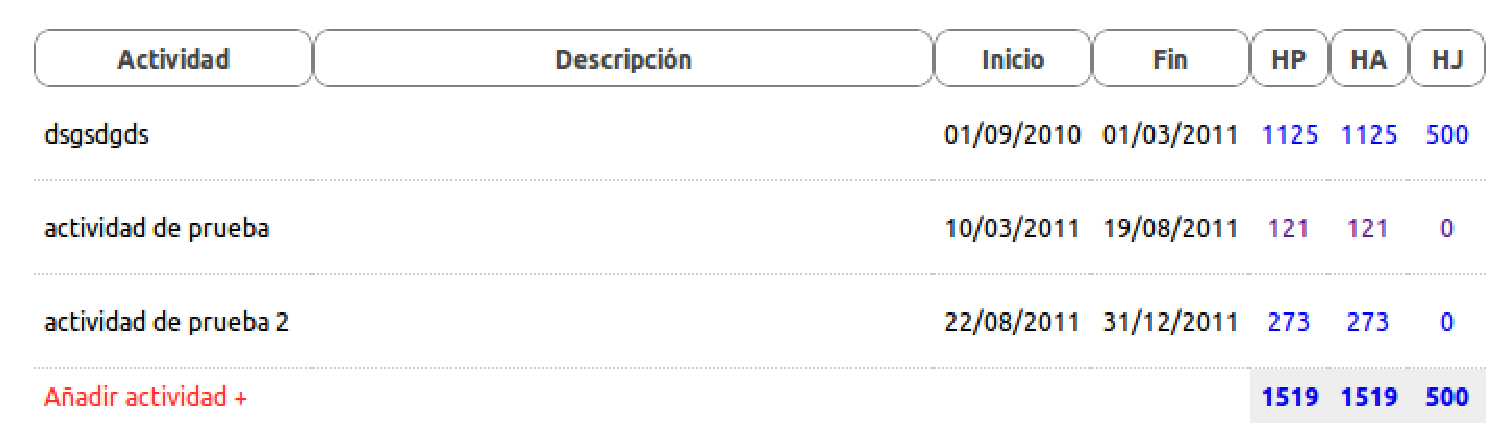
\epsfig{file=imagenes/manual/consulta_horas_act.eps,width=5.28in}
\caption{Desglose general por actividades.}
\label{fig:consulta_horas_act}
\end{figure}

\begin{figure}
\centering
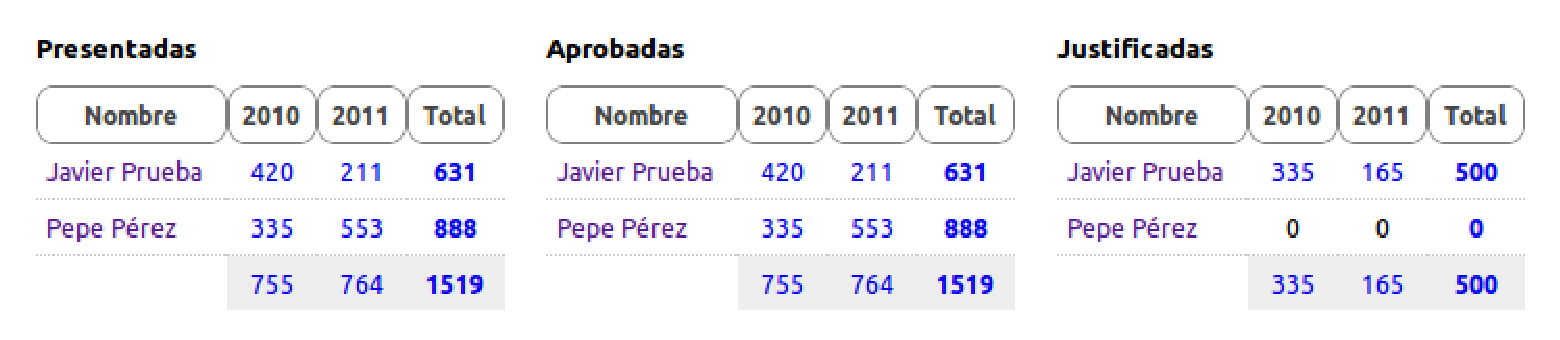
\epsfig{file=imagenes/manual/horas_resumen_anio.eps,width=5.28in}
\caption{Resumen de horas por año.}
\label{fig:horas_resumen_anio}
\end{figure}

\begin{figure}
\centering
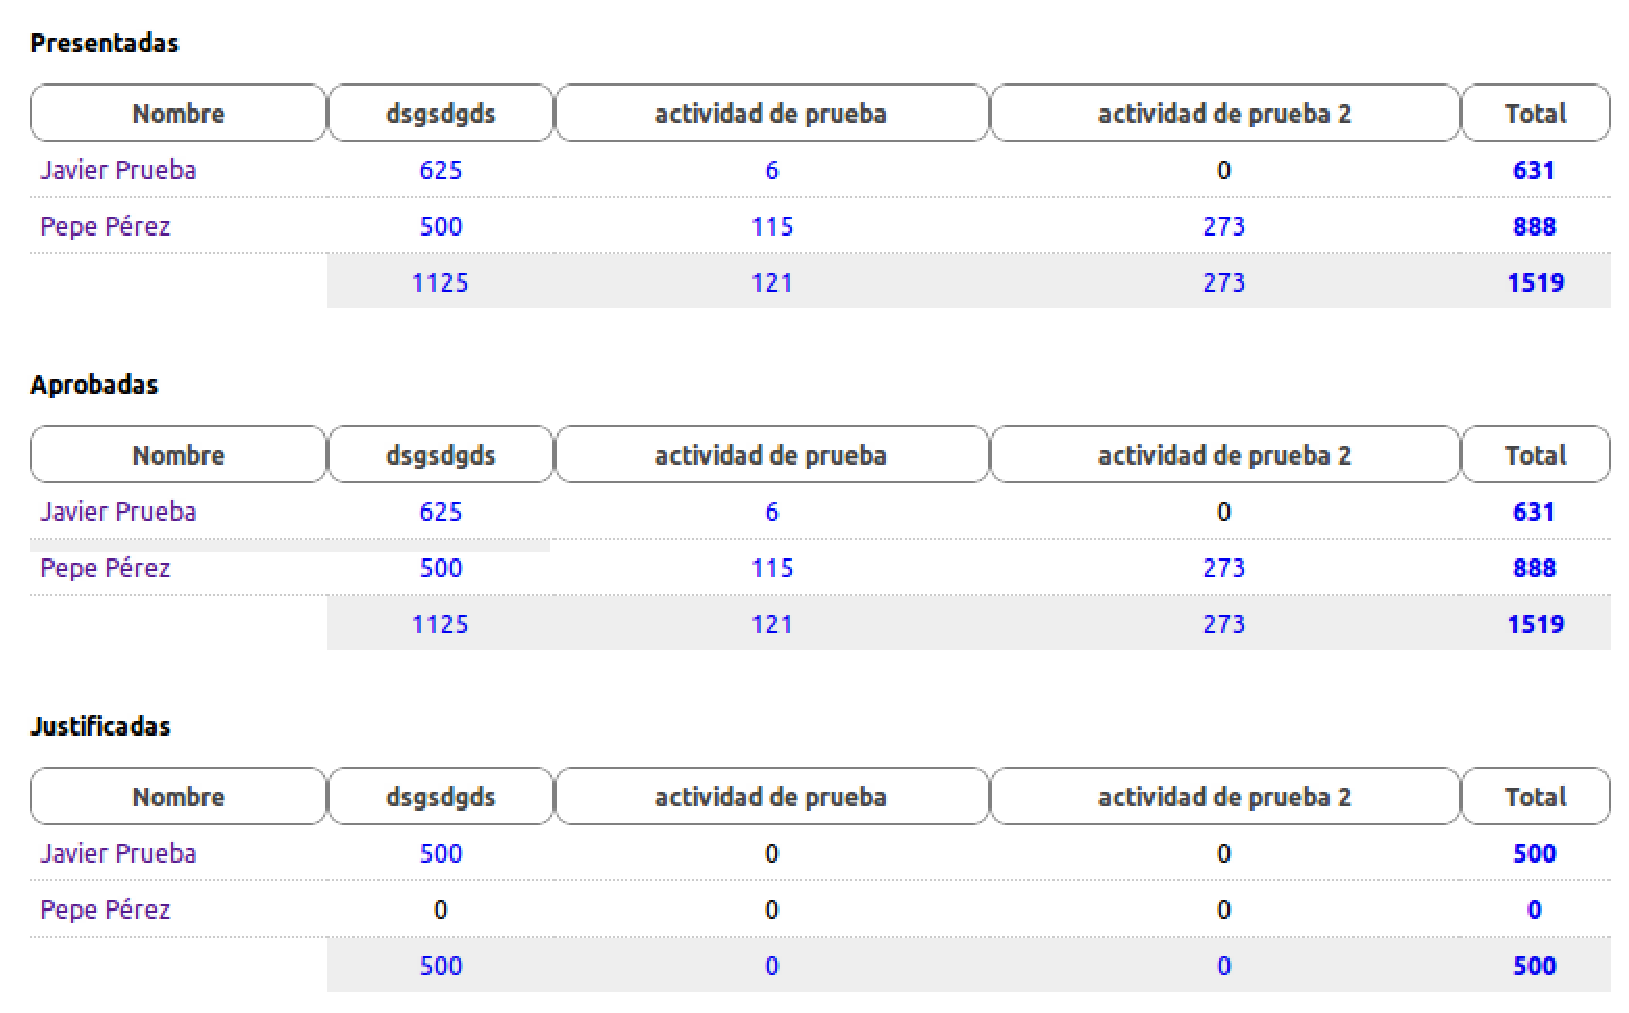
\epsfig{file=imagenes/manual/horas_resumen_actividad.eps,width=5.28in}
\caption{Resumen de horas por año.}
\label{fig:horas_resumen_actividad}
\end{figure}

A partir de los enlaces de cada valor, podemos acceder al desglose mensual
(figura \ref{fig:desglose_horas}) y ajustar el filtro para nuestras necesidades
en cada momento; así, por ejemplo, podríamos seleccionar todos los empleados y
un proyecto o actividades concretos.

Adicionalmente, existe la posibilidad de descargar (figura
\ref{fig:enlace_resumen}) una hoja de cálculo con la información de cada
empleado acerca de su participación en el proyecto para su etapa de
presentación, aprobación o justificación. La hoja de cálculo tiene tantas hojas
como empleados participan en el proyecto, y tiene el aspecto de la figura
\ref{fig:hoja_calculo_proyecto}.

\begin{figure}
\centering
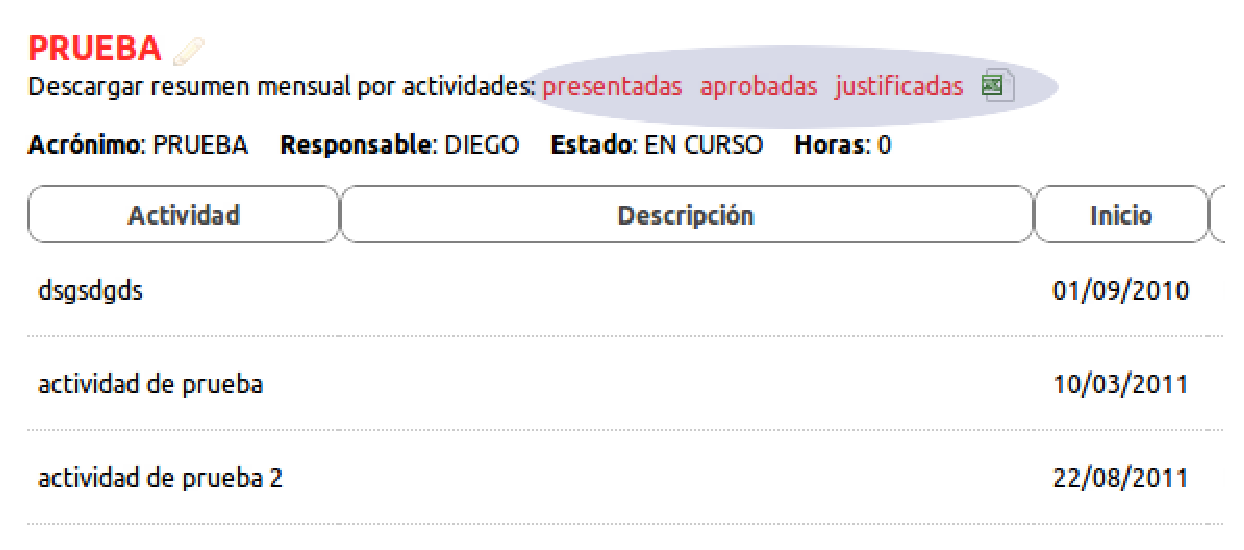
\epsfig{file=imagenes/manual/enlace_resumen.eps,width=5.28in}
\caption{Enlace a las hojas de cálculo.}
\label{fig:enlace_resumen}
\end{figure}

\begin{figure}
\centering
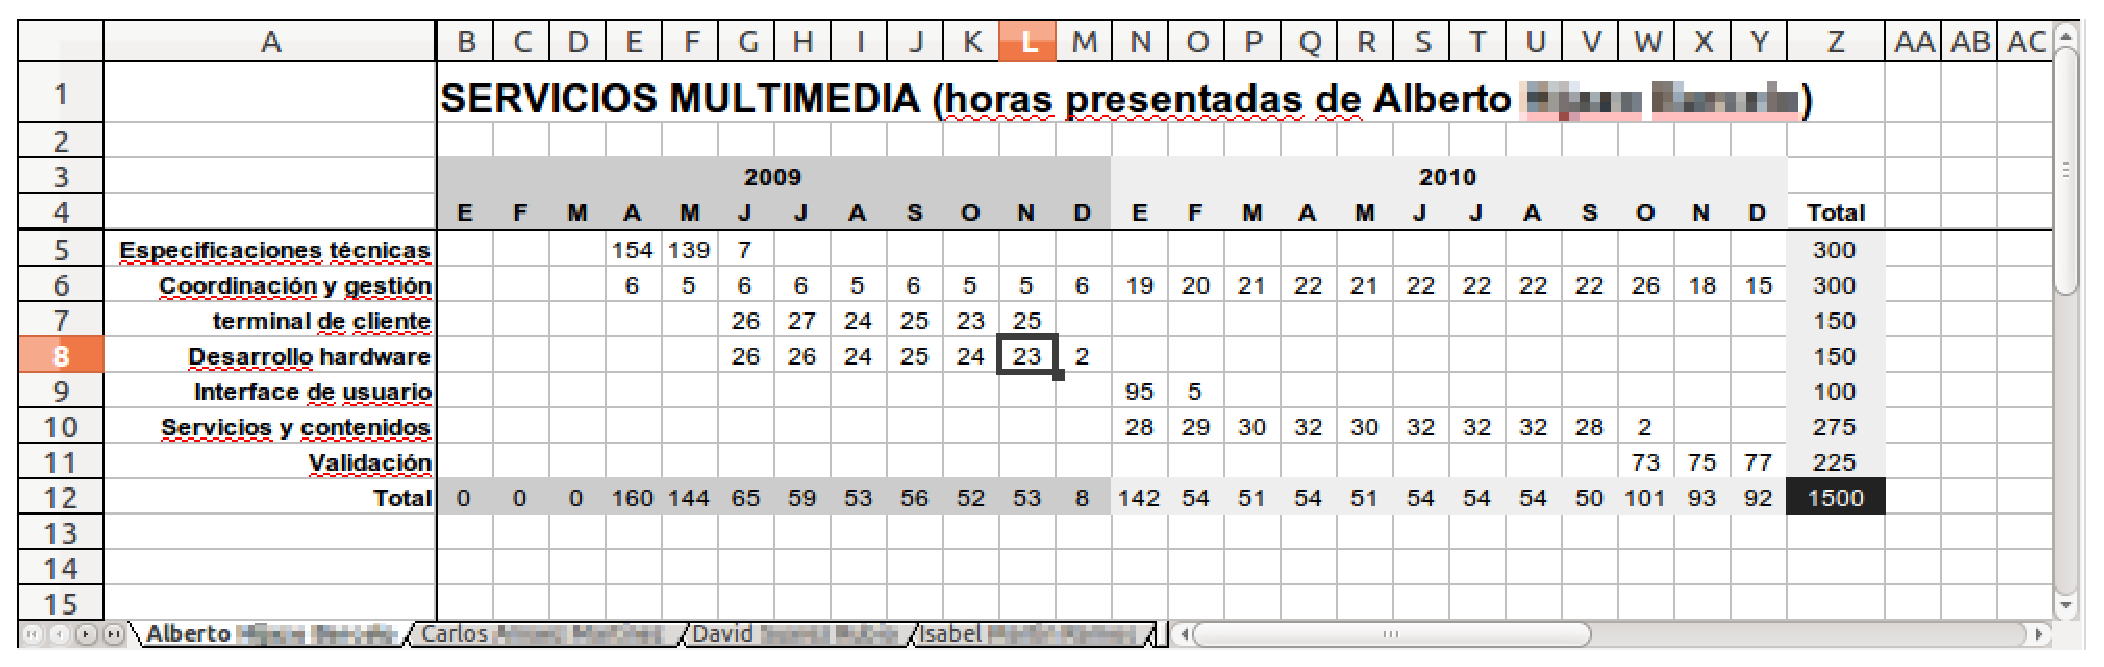
\epsfig{file=imagenes/manual/hoja_calculo_proyecto.eps,width=5.28in}
\caption{Hoja de cálculo por proyecto, personal, actividades y meses.}
\label{fig:hoja_calculo_proyecto}
\end{figure}

\subsection{Resumen global}

Se puede acceder a un resumen global desde cualquier parte de los módulos de
\textbf{Personal} y \textbf{Actividades}, como se ve en la figura
\ref{fig:enlace_resumen_global_mont}, desde la que también se aprecia que se
puede pasar fácilmente de las actividades de un cliente a su personal y
viceversa.

\begin{figure}
\centering
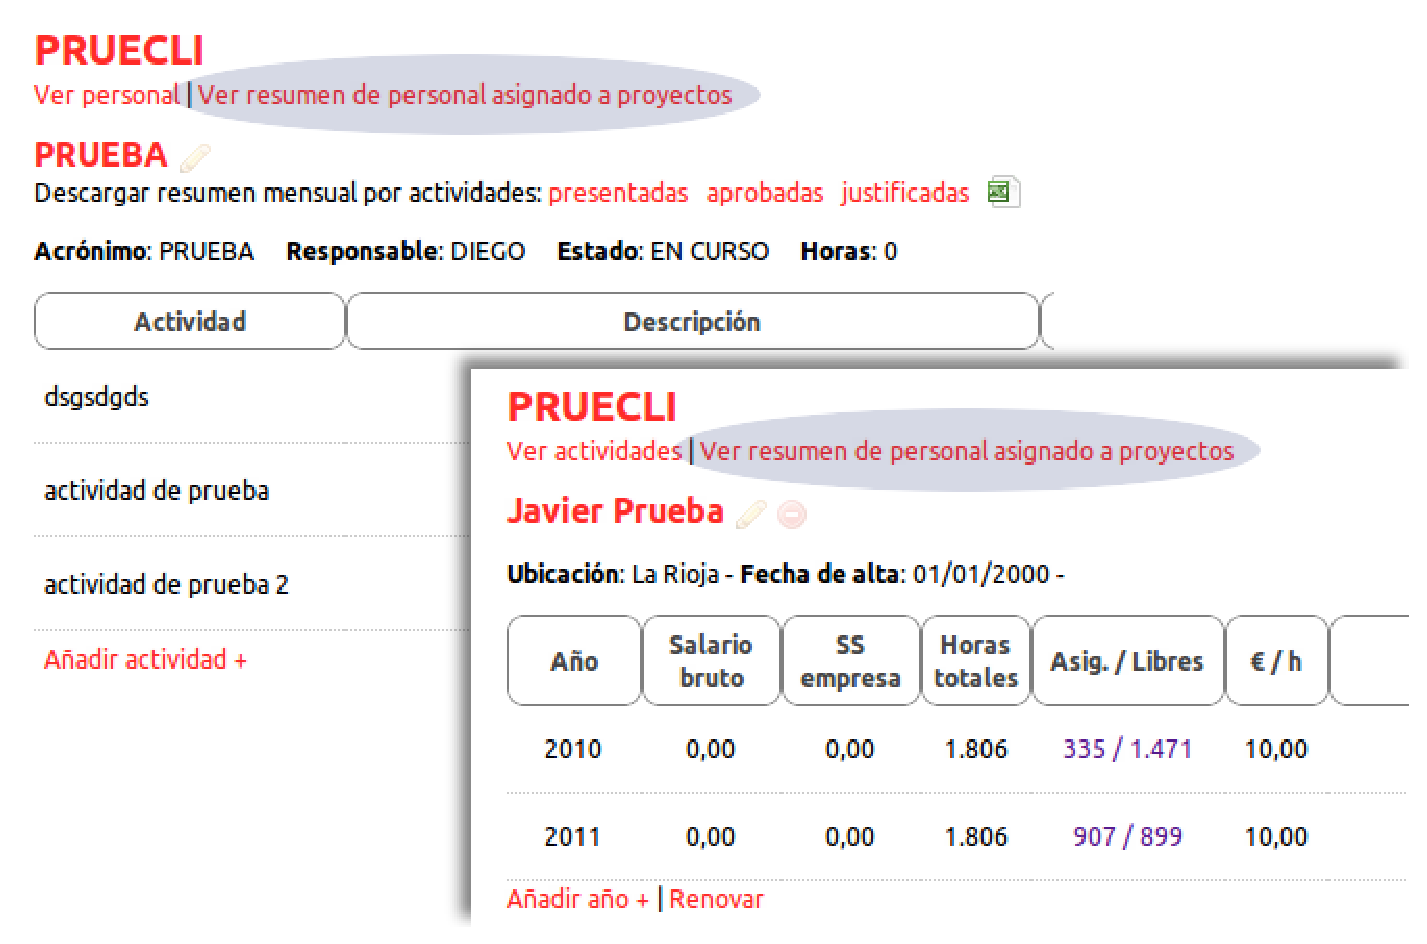
\epsfig{file=imagenes/manual/enlace_resumen_global_mont.eps,width=5.28in}
\caption{Enlaces al resumen desde Proyectos (izq.) y personal (dcha.).}
\label{fig:enlace_resumen_global_mont}
\end{figure}

El objetivo del resumen global (figura
\ref{fig:resumen_horas_asignadas_proyectos}) es que sea posible, de un vistazo,
obtener la mayor cantidad de información posible:

\begin{itemize}
\item puede identificarse cuándo un empleado no está dado de alta en la
empresa.

\item se tiene en cuenta el convenio de horas del recurso para informar acerca
de las horas que le quedan libres en un año;

\item cuando existe un conflicto, por ejemplo, se hayan imputado más horas
de las que deberían, el valor aparece marcado en rojo;

\item las columnas de proyectos siguen un código de colores para indicar el
estado en que se encuentra el proyecto;

\item cada uno de los valores, incluidos los nombres de los recursos en
cuestión, son un enlace a otra vista donde se darán detalles acerca
del elemento (la figura \ref{fig:desglose_mensual_actividades} es el desglose
de las horas marcadas en la figura \ref{fig:resumen_horas_asignadas_proyectos}).
En esta vista, también se muestra el coste/hora de
cada empleado para calcular el coste de la selección.
\end{itemize}

\begin{figure}
\centering
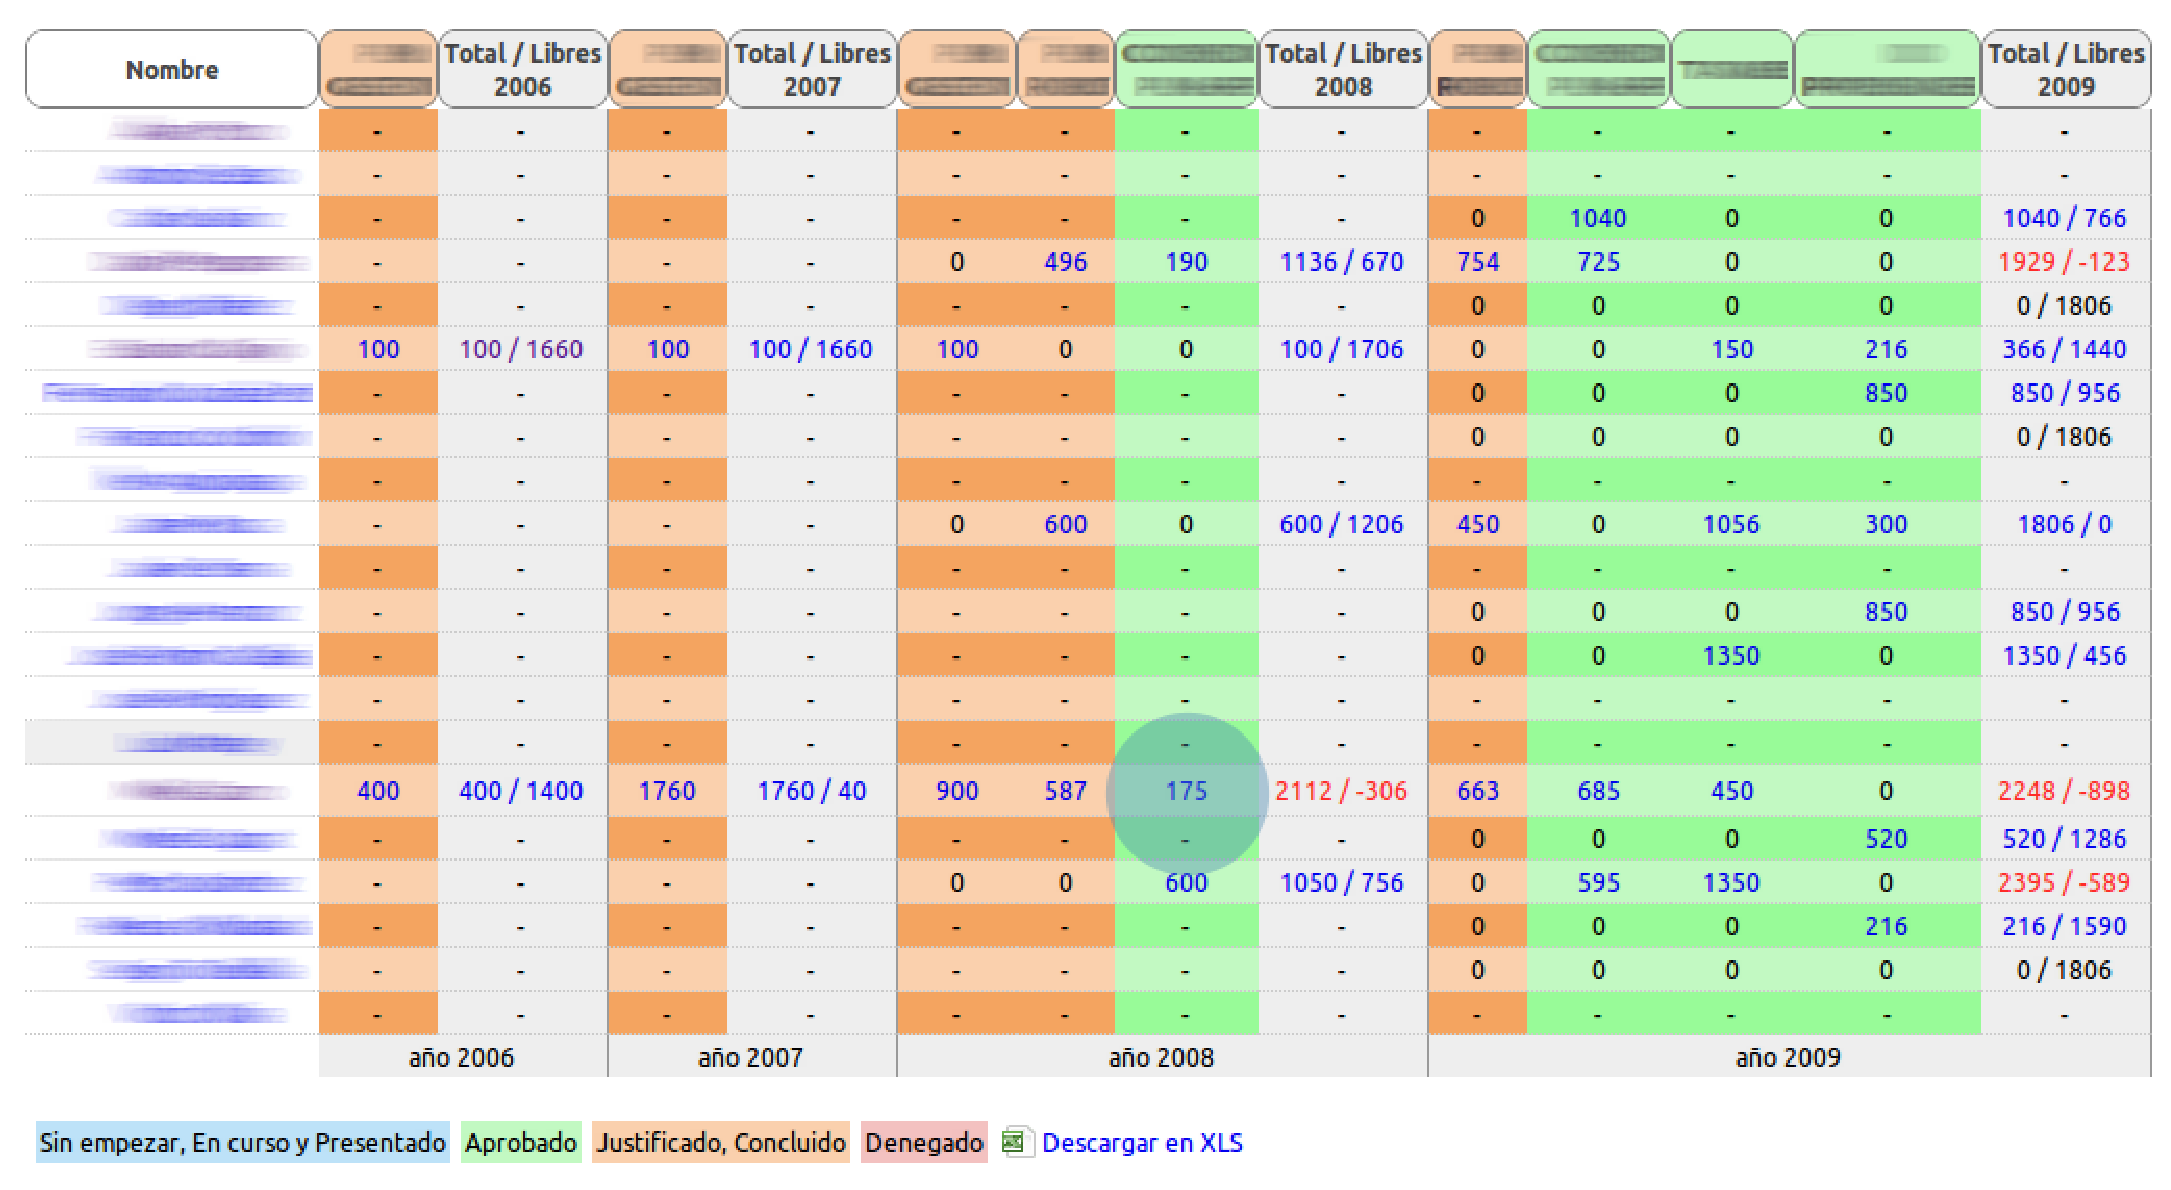
\epsfig{file=imagenes/manual/prediccion_resumen.eps,width=5.28in}
\caption{Resumen de horas asignadas a proyectos.}
\label{fig:resumen_horas_asignadas_proyectos}
\end{figure}

\begin{figure}
\centering
\epsfig{file=imagenes/manual/desglose_mensual_actividades.eps,width=5.28in}
\caption{Vista de desglose mensual por actividades.}
\label{fig:desglose_mensual_actividades}
\end{figure}

El resumen global puede descargarse en formato de hoja de cálculo desde el
enlace que figura junto a la leyenda bajo la tabla en sí, y tiene el aspecto de
la figura \ref{fig:hoja_calculo_global}.

\begin{figure}
\centering
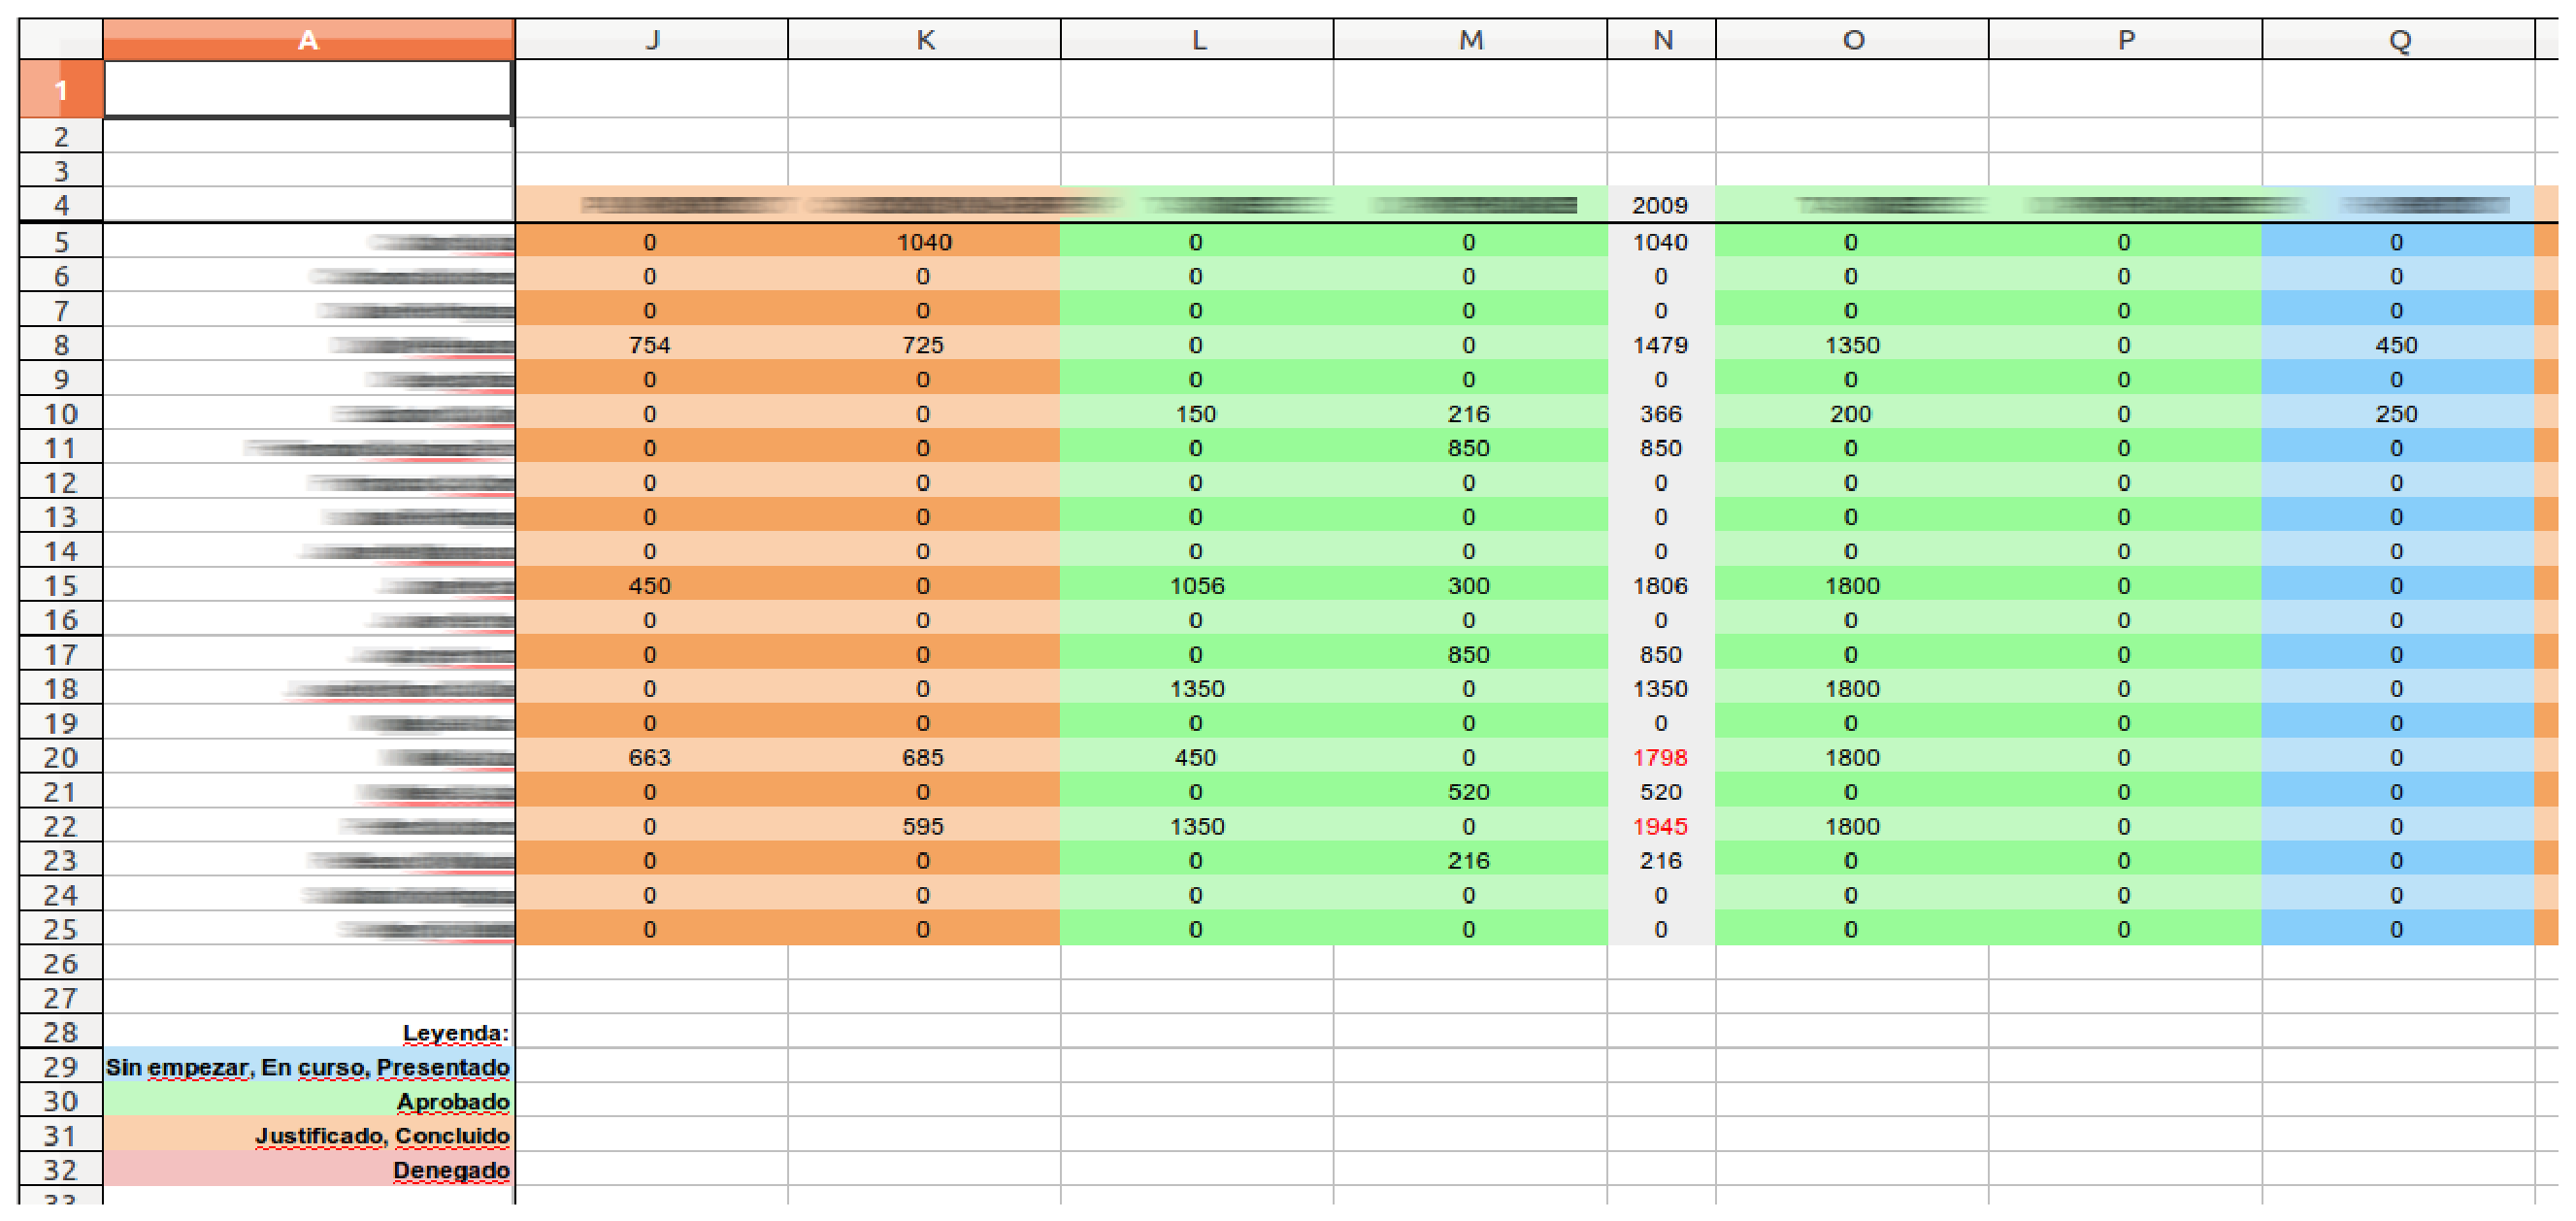
\epsfig{file=imagenes/manual/hoja_calculo_global.eps,width=5.28in}
\caption{Resumen global en hoja de cálculo.}
\label{fig:hoja_calculo_global}
\end{figure}

\section{Gestión de horas}
\label{sec:manual_horas}

\subsection{Asignación de horas}

La imputación efectiva de horas se realiza desde el módulo de actividades,
pinchando en el icono que representa a una persona a la derecha de la tabla de
actividades de cada proyecto (figura \ref{fig:asig_horas}).

\begin{figure}
\centering
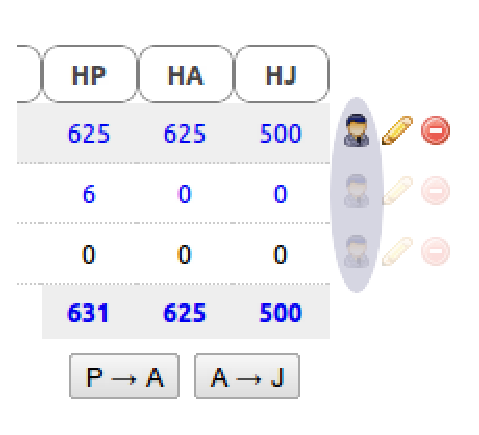
\epsfig{file=imagenes/manual/asig_horas.eps,width=2.23in}
\caption{Enlace para imputar horas a una actividad.}
\label{fig:asig_horas}
\end{figure}

El formulario de asignación (figura \ref{fig:form_asig_horas}) requiere los
siguientes datos para realizar correctamente la imputación:

\begin{description}
 \item [Persona] Se trata del empleado a quien se desea imputar horas. Se
puede elegir entre un listado que comprende a los empleados del cliente
responsable del proyecto y a los de todos los clientes que figuran como
cooperantes del proyecto.
 \item [Tipo de horas] Se refiere a la naturaleza de las horas a imputar:
presentadas, aprobadas o justificadas.
 \item [Inicio] Se refiere al inicio de las acciones del empleado en la
actividad. Por defecto, se considera la fecha de inicio de la actividad.
 \item [Fin] Se refiere al fin de las acciones del empleado en la
actividad. Por defecto, se considera la fecha de fin de la actividad.
\end{description}

\begin{figure}
\centering
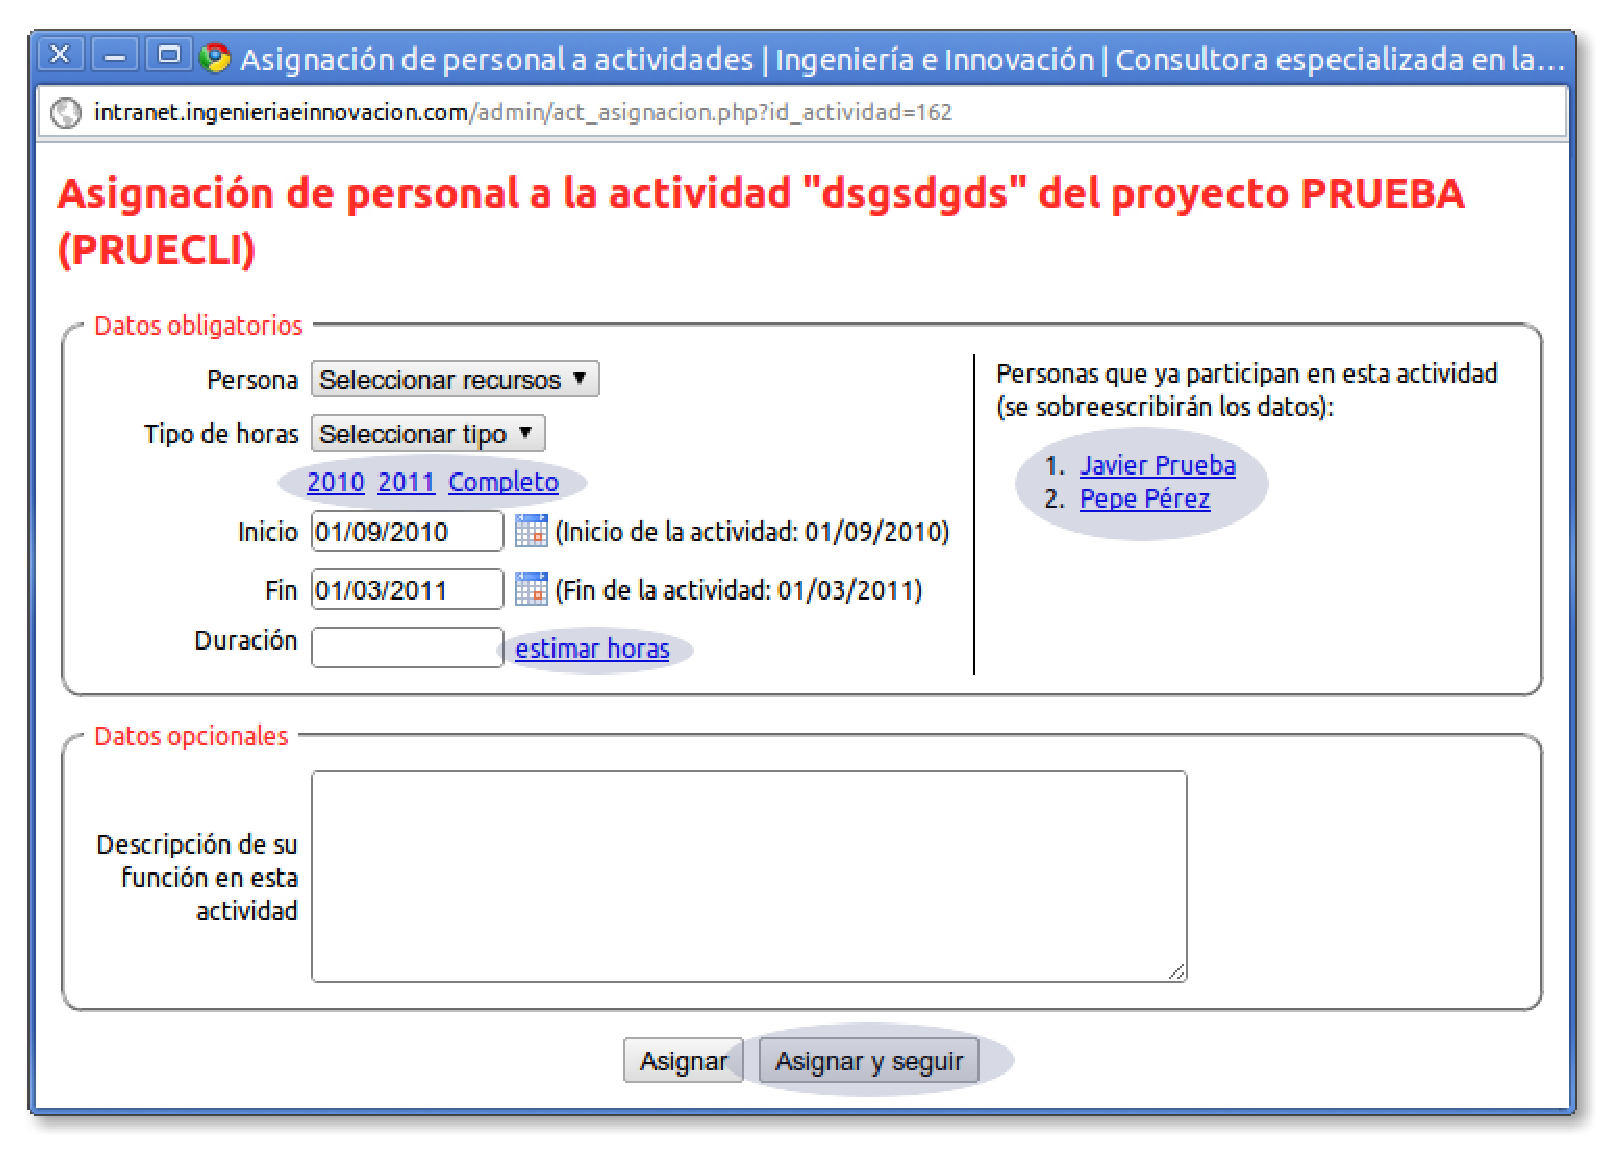
\epsfig{file=imagenes/manual/form_asig_horas.eps,width=5.28in}
\caption{Formulario de asignación de horas a actividad.}
\label{fig:form_asig_horas}
\end{figure}

Sobre el formulario de asignación (figura \ref{fig:form_asig_horas}), se pueden
destacar algunas cosas:

\begin{itemize}
 \item nos da un listado
de los empleados que ya tienen horas imputadas, de manera que se reduzca la
posibilidad duplicar el esfuerzo;
 \item cuando el inicio y final de la actividad se extiende durante varios
años, nos permite, con un clic, seleccionar el año concreto al que queremos
asignar horas.
 \item nos ayuda a calcular el número de horas basándose en el calendario real
de trabajo (teniendo en cuente festivos...) a partir del número de horas que se
calcula que el trabajador empleará al día en esa actividad.
 \item la opción \textit{asignar y seguir} envía los valores pero mantiene el
formulario abierto con los mismos valores. Esto es especialmente útil cuando
estamos asignando horas en la misma actividad a varios empleados.
\end{itemize}

Dado que en muchas ocasiones se aprueban tantas horas como se presentan o
se justifican tantas como se aprueban, existe la posibilidad de trasladar unas
horas al siguiente estado sin necesidad de reasignar las horas de cada empleado.
Esta acción solamente requiere un clic en los botones correspondientes bajo la
lista de actividades (figura \ref{fig:tras_horas}) pero, ya que sobrescribe
cualquier valor que hubiera previamente, solo puede ser ejecutada por el
administrador.

\begin{figure}
\centering
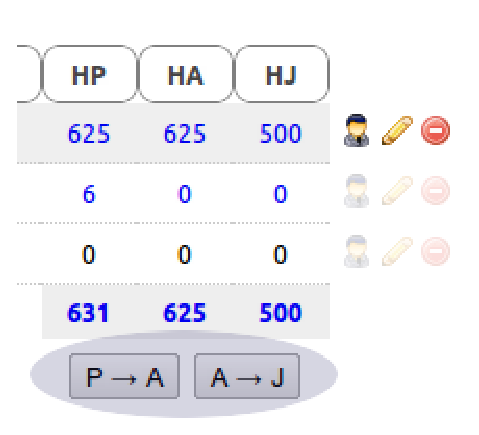
\epsfig{file=imagenes/manual/tras_horas.eps,width=2.23in}
\caption{Botones de traslación de horas.}
\label{fig:tras_horas}
\end{figure}

\subsection{Modificación de horas asignadas}

El método más simple que tenemos para modificar las horas asignadas a un
empleado es sobrescribir, es decir, hacer una asignación sobre un periodo de
tiempo que ya tenía horas asignadas. Otra acción que nos permite realizar la
aplicación es modificar la asignación mensual calculada automáticamente. Para
ello, debemos acceder a la vista de horas por meses desde cualquier enlace de
horas de los módulos de personal o actividades. Una vez allí, basta con pinchar
en cualquier valor por mes para realizar la modificación, como se ve en la
figura \ref{fig:mod_horas_mes}.

\begin{figure}
\centering
\epsfig{file=imagenes/manual/mod_horas_mes.eps,width=4in}
\caption{Modificación de horas mensuales.}
\label{fig:mod_horas_mes}
\end{figure}

La modificación mensual es muy útil para resolver manualmente las
inconsistencias que pudieran haberse creado en los procesos de asignación.

Debe tenerse en cuenta que no pueden asignarse o modificarse horas
\textit{presentadas} a proyectos \textit{aprobados}, ni horas
\textit{presentadas} o \textit{aprobadas} a proyectos \textit{justificados}.
Cuando un proyecto está \textit{concluido}, no se pueden asignar o modificar
horas de ningún tipo.

\subsection{Detección de errores}

La detección de errores no requiere de ninguna acción por parte del usuario.
Cualquier inconsistencia es marcada en rojo automáticamente, a la espera de las
acciones correctoras de los técnicos.

Ya en la propia asignación de horas, el sistema advierte de cuáles son las
inconsistencias que la acción ha provocado. Se puede ver un ejemplo de esto en
la figura \ref{fig:errores_detectados}.

\begin{figure}
\centering
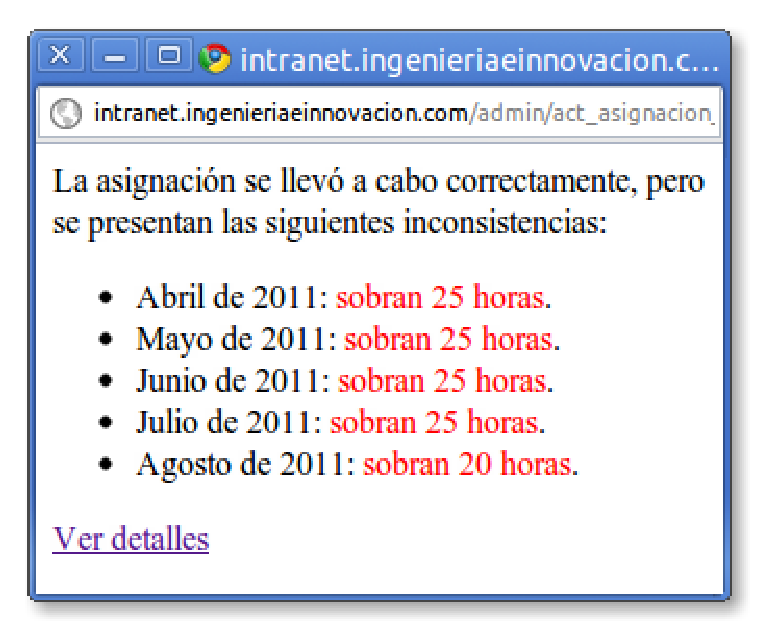
\epsfig{file=imagenes/manual/errores_detectados.eps,width=3in}
\caption{Detección de errores en la asignación.}
\label{fig:errores_detectados}
\end{figure}

Al pinchar en el enlace para ver los detalles, se nos muestra el filtro general
con las opciones apropiadas preseleccionadas para ver los valores en cuestión.
La última columna de la figura \ref{fig:detalles_errores} muestra las horas
sobrantes y nos enlaza al mes en cuestión, independientemente del proyecto, de
manera que sea posible identificar la naturaleza de la inconsistencia: por
ejemplo, solapamiento del trabajo del empleado en varios proyectos.

\begin{figure}
\centering
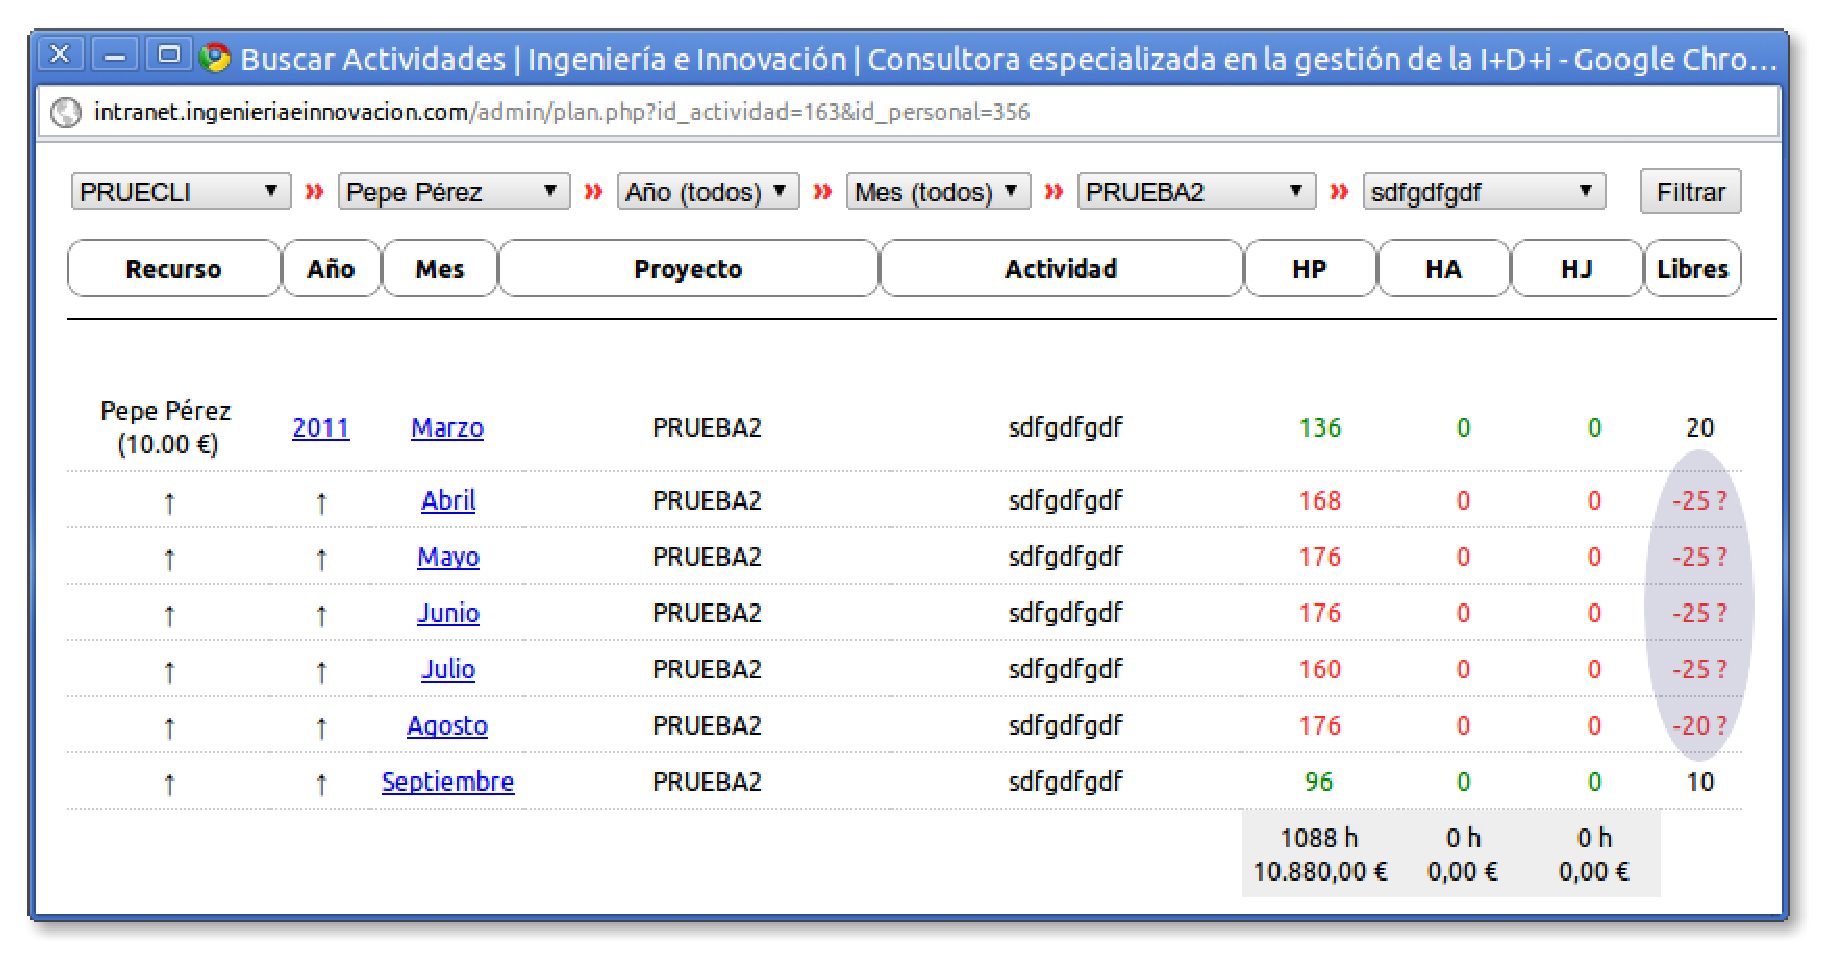
\epsfig{file=imagenes/manual/detalles_errores.eps,width=5.28in}
\caption{Detalle de los errores con enlace de horas sobrantes.}
\label{fig:detalles_errores}
\end{figure}

\subsection{Eliminación de horas asignadas}

La eliminación de horas asignadas se realiza sobrescribiendo las horas a
eliminar con una asignación de cero horas. Asimismo, pueden eliminarse meses
concretos desde la vista de desglose mensual (figura \ref{fig:mod_horas_mes}),
de nuevo, mediante la asignación de cero horas.

Cualquier eliminación de personal involucrado en un proyecto o de actividades
que se lleven a cabo en el marco del proyecto eliminan, por supuesto, sus
correspondientes horas asignadas.

\section{Buscador global}

El buscador global es la página de inicio de la aplicación, y también está
disponible a lo largo de toda la sesión en la barra de menú superior (figuras
\ref{fig:buscador_inicio} y \ref{fig:buscador_superior}).

\begin{figure}
\centering
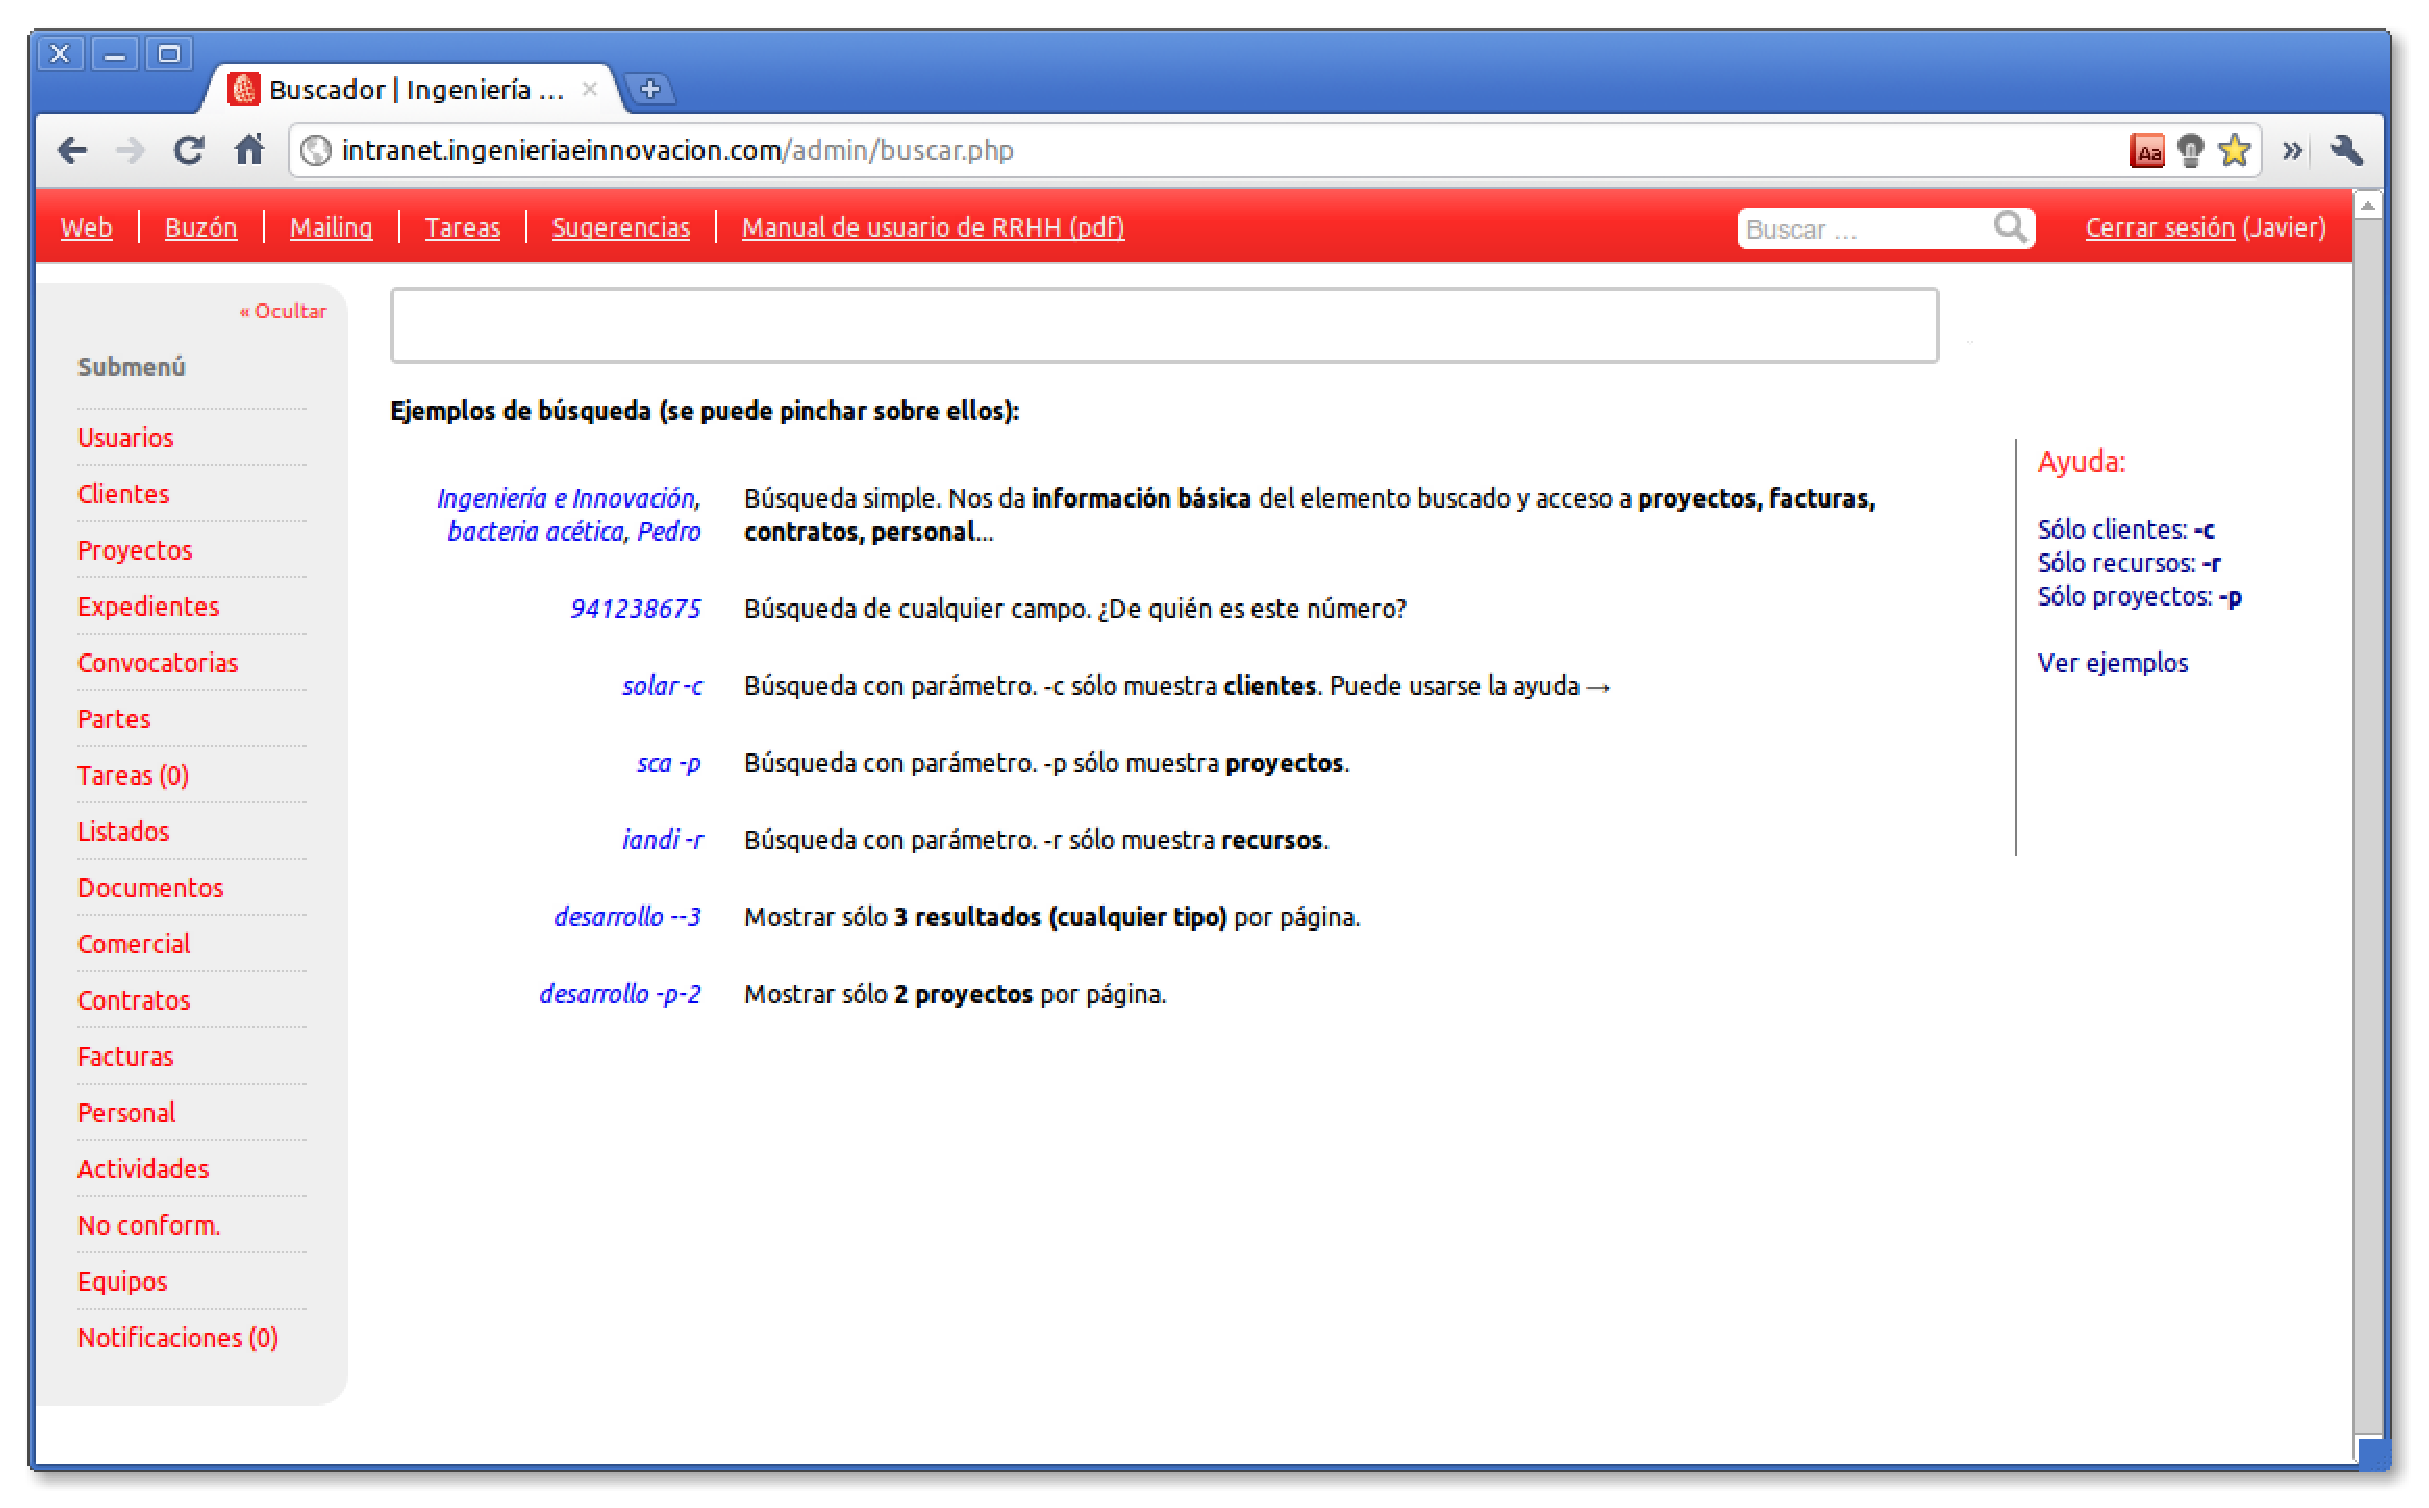
\epsfig{file=imagenes/manual/buscador_inicio.eps,width=5.28in}
\caption{Buscador con ejemplos de uso.}
\label{fig:buscador_inicio}
\end{figure}

\begin{figure}
\centering

\epsfig{file=imagenes/manual/buscador_superior.eps,width=5.28in}
\caption{Posición del buscador en el menú superior.}
\label{fig:buscador_superior}
\end{figure}

Nos permite buscar clientes, recursos humanos y proyectos. Su funcionalidad
general puede describirse con los ejemplos del cuadro
\ref{cua:buscador_opciones}. Para buscar, solamente es necesario comenzar a
teclear en la caja del buscador; los resultados irán apareciendo y
actualizándose mientras sigamos tecleando.

\begin{table}
\centering
\begin{tabular}{|p{1.28in}|p{4in}|}\hline
Consulta & Descripción / Resultado \\\hline\hline
Ingeniería e Innovación, bacteria acética, Pedro & Búsqueda simple. Nos da
información básica del elemento buscado y acceso a proyectos, facturas,
contratos, personal...\\\hline
941238675 & Búsqueda de cualquier campo. ¿De quién es este número?\\\hline
solar -c & Búsqueda con parámetro. -c sólo muestra clientes.\\\hline
soluciones -p & Búsqueda con parámetro. -p sólo muestra proyectos.\\\hline
iandi -r & Búsqueda con parámetro. -r sólo muestra recursos.\\\hline
desarrollo --3 & Mostrar sólo 3 resultados (cualquier tipo) por página.\\\hline
desarrollo -p-2 & Mostrar sólo 2 proyectos por página.\\\hline
\end{tabular}
\caption{Listado de ejemplos de búsqueda característicos.}
\label{cua:buscador_opciones}
\end{table}

La interfaz es muy similar a la de cualquier buscador web, y también la forma
de interactuar con ella. La paginación se puede controlar tanto desde la
parte superior, debajo de la caja de búsqueda, como desde la parte inferior. El
número de resultados y el tiempo que ha costado reunirlos también se puede
consultar debajo de la caja de búsqueda. Otros elementos a tener en cuenta son
las etiquetas acerca del tipo de elemento, junto al título del resultado y los
enlaces de interés a proyectos, facturas, personal... Todos estos elementos
pueden verse en la figura \ref{fig:buscador_elementos}.

El buscador trata de mostrar los resultados más interesantes. Así, entre todos
los elementos que satisfacen la consulta, primero se muestran los clientes,
después los recursos humanos y por último, los proyectos. Además, dentro de los
clientes y de los proyectos, se muestran primero los que se consideran más
importantes teniendo en cuenta el número de proyectos del cliente y el número
de expedientes del proyecto. Los recursos humanos se listan por orden
alfabético.

Como se puede ver en el cuadro \ref{cua:buscador_opciones}, el buscador cuenta
con una serie de funciones básicas para configurar los resultados. Para coger
soltura con estas funciones, lo mejor es probarlas y ver como podemos sacar
mejor partido de ellas.

Si no queremos recordar que \textit{-p} nos mostrará solamente proyectos,
podemos hacer uso de la ayuda que se muestra junto a los resultados y pinchar
sobre esa opción (figura \ref{fig:buscador_ayuda}). Esto adaptará los
resultados a nuestras necesidades cuando nos cueste encontrar lo que buscamos.

Otra característica importante del buscador, y que resulta muy útil a pesar de
ser muy simple, es que, cuando no encuentra resultados, es capaz de ir
truncando la consulta letra por letra por si el usuario ha cometido algún error
tipográfico. De esta forma, si encuentra algún resultado usando más de tres
letras de la consulta original, muestra un mensaje indicando la parte que
coincide y los resultados asociados, como puede apreciarse en la figura
\ref{fig:buscador_cercanos}.

La última característica que requiere mención especial es que se permite la
navegación por teclado, de modo que la flecha derecha ($\rightarrow$) pasa a la
siguiente página y la flecha izquierda ($\leftarrow$), a la anterior.

\begin{figure}
\centering
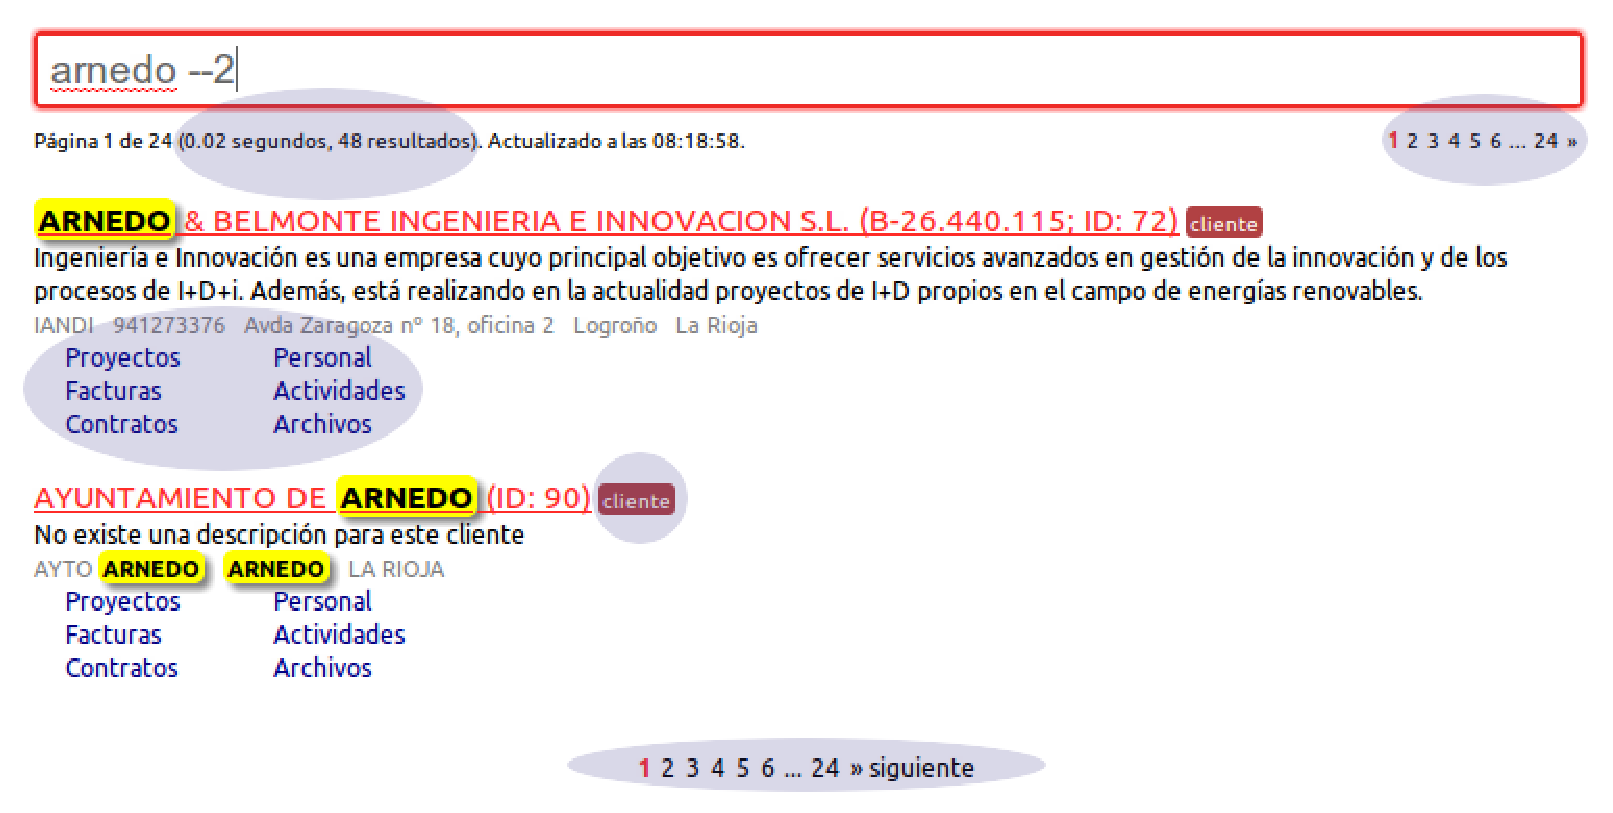
\epsfig{file=imagenes/manual/buscador_elementos.eps,width=5.28in}
\caption{Elementos principales de una búsqueda.}
\label{fig:buscador_elementos}
\end{figure}

\begin{figure}
\centering
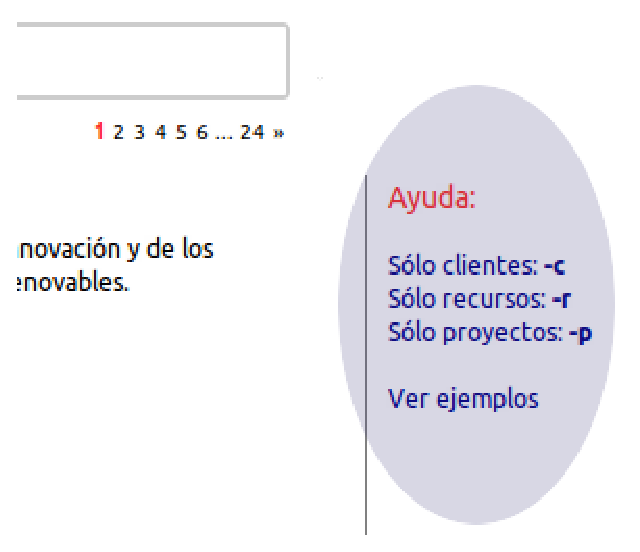
\epsfig{file=imagenes/manual/buscador_ayuda.eps,width=3in}
\caption{Menú de ayuda del buscador.}
\label{fig:buscador_ayuda}
\end{figure}

\begin{figure}
\centering
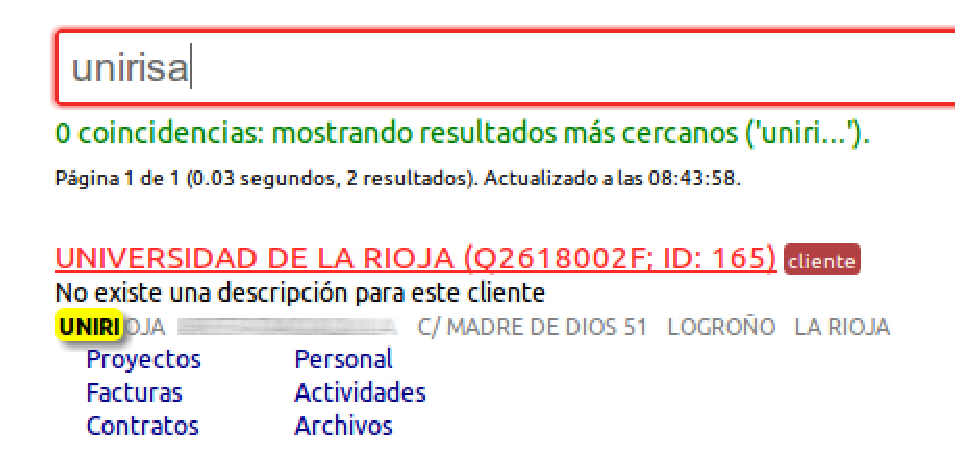
\epsfig{file=imagenes/manual/buscador_cercanos.eps,width=4.5in}
\caption{Búsqueda de elementos cercanos.}
\label{fig:buscador_cercanos}
\end{figure}
